\documentclass[12pt]{article}

% Keep the PDF trailer identifier stable across isolated reproducible builds.
\ifdefined\pdftrailerid
  \pdftrailerid{0123456789ABCDEF0123456789ABCDEF}
\fi

\usepackage[margin=1in]{geometry}
% \usepackage{newtxtext,newtxmath}
% \usepackage[T1]{fontenc}
% \usepackage[utf8]{inputenc}
\usepackage{textcomp}
\usepackage{microtype}
\usepackage{amsmath,mathtools,amssymb,bbm}
\usepackage{booktabs,tabularx,array}
\usepackage[most]{tcolorbox}
\usepackage{listings}
\usepackage{enumitem}
\usepackage{graphicx}
\usepackage{caption}
\usepackage[titles]{tocloft}
\setlength{\cftbeforesecskip}{3pt}
\usepackage{tikz}
\usetikzlibrary{positioning,backgrounds,fit,calc,decorations.pathreplacing}
\usepackage{xcolor}
\usepackage{fancyhdr}
\usepackage{lastpage}
\usepackage{hyperref}
\usepackage{xurl}
\usepackage{cleveref}

\definecolor{ink}{HTML}{24292F}
\definecolor{blue}{HTML}{0969DA}
\definecolor{green}{HTML}{1A7F37}
\definecolor{orange}{HTML}{9A6700}
\definecolor{purple}{HTML}{8250DF}
\definecolor{gray}{HTML}{57606A}
\definecolor{codebg}{HTML}{F6F8FA}
\definecolor{codeborder}{HTML}{D0D7DE}
% \alert{...}: dark blue and underlined, as in the guest-lecture slides;
% \uline (ulem) lets the underline break across lines.
\usepackage[normalem]{ulem}
\definecolor{alertblue}{HTML}{1F4E79}
\newcommand{\alert}[1]{{\color{alertblue}\uline{#1}}}

\hypersetup{colorlinks=true,linkcolor=green,citecolor=green,urlcolor=green,
  pdftitle={Data-Center Connection Planning Game: Assignment and Student Tutorial},
  pdfauthor={ECE 51032, Purdue University}}

\lstdefinestyle{tutorialcode}{basicstyle=\ttfamily\small,backgroundcolor=\color{codebg},
  frame=single,rulecolor=\color{codeborder},framerule=0.5pt,columns=fullflexible,
  keepspaces=true,breaklines=true,breakatwhitespace=false,breakautoindent=true,
  postbreak=\mbox{\textcolor{gray}{$\hookrightarrow$\space}},showstringspaces=false,
  xleftmargin=0.5em,xrightmargin=0.5em}
\lstset{style=tutorialcode}
% Syntax colors (GitHub light palette) for language=python and language=bash.
\definecolor{codekeyword}{HTML}{CF222E}
\definecolor{codestring}{HTML}{0A3069}
\definecolor{codecomment}{HTML}{6E7781}
\definecolor{codebuiltin}{HTML}{8250DF}
\lstset{keywordstyle=\color{codekeyword}\bfseries,
  stringstyle=\color{codestring},
  commentstyle=\color{codecomment}\itshape,
  emphstyle=\color{codebuiltin}}
\lstdefinelanguage{tutorialpython}[]{Python}{
  morekeywords={as,with,None,True,False},
  emph={print,len,round,range,open,str,int,float,list,dict,sorted,sum,min,max}}
\lstdefinestyle{csvfile}{style=tutorialcode,basicstyle=\ttfamily\scriptsize,
  breaklines=false,postbreak=\mbox{}}

% Four box types: a key idea, a pitfall, an exercise, and a prompt to give an AI.
\tcbset{tutorialbox/.style={breakable,fonttitle=\bfseries\small,boxrule=0.6pt,arc=2pt,
  left=6pt,right=6pt,top=4pt,bottom=4pt}}
\newtcolorbox{keybox}[1][Key idea]{tutorialbox,colback=blue!4,colframe=blue!70!black,title={#1}}
\newtcolorbox{warningbox}[1][Watch out]{tutorialbox,colback=orange!6,colframe=orange!85!black,title={#1}}
\newtcolorbox{exercisebox}[1][Try it]{tutorialbox,colback=purple!4,colframe=purple!70!black,title={#1}}
\newtcolorbox{promptbox}[1][Ask AI]{tutorialbox,colback=green!4,colframe=green!60!black,title={#1}}
\newtcolorbox{aibox}[1][Example AI reply]{tutorialbox,colback=gray!5,colframe=gray!70!black,title={#1}}

\pagestyle{fancy}
\setlength{\headheight}{15pt}
\fancyhf{}
\lhead{Data-Center Connection Planning Game}
\rhead{Assignment and Tutorial}
\cfoot{\thepage\ of \pageref{LastPage}}
\newcommand{\code}[1]{\path{#1}}
% Literal text that contains spaces (\path drops them).
\newcommand{\msg}[1]{\texttt{\detokenize{#1}}}
\newcommand{\MW}{\ensuremath{\,\mathrm{MW}}}
\newcommand{\MWh}{\ensuremath{\,\mathrm{MWh}}}
% Placeholder for a decision the instructor still has to fill in.
\newcommand{\instr}[1]{\textcolor{red}{\textbf{[Instructor: #1]}}}
% Unnumbered page heading in Part I that still appears in the table of contents.
\newcommand{\assignsection}[2]{\section*{#1}\phantomsection\addcontentsline{toc}{section}{#1}\label{#2}}
\setlength{\parindent}{0pt}
\setlength{\parskip}{0.55em}
\emergencystretch=3em
\captionsetup{font=small,labelfont=bf}
\setlist{itemsep=2pt,topsep=3pt}

\title{\vspace{-2em}ECE 51032: Computational Methods for Power System Analysis\\ \textbf{Data-Center Connection Planning Game}\\[0.3em]\large Assignment and Student Tutorial}
\date{Fall 2026}
\author{Purdue University}
\begin{document}
\maketitle

This document has two parts. \textbf{Part I} is the official
assignment: the rules, the scoring, what you submit, and how it is graded. \textbf{Part II} is the tutorial: it explains the game, the model,
the tools, and strategy, and walks you through your first plan.

\phantomsection\addcontentsline{toc}{part}{Part I: The Assignment}
\begin{center}
\Large\bfseries Part I: The Assignment
\end{center}

% ---------------------------------------------------------------------------
\assignsection{Assignment at a glance}{asg:glance}

\paragraph{Your role.} Your team is a data-center operator in Texas. Each week
you decide where to connect computing load to a model of the Texas grid, how
many MW to request at each site, and whether to build a private generator or
battery next to it. The instructor, acting as the grid operator, dispatches
every team's plan together on the same network and scores each team in
dollars. Your goal is the highest total score over the graded weeks.

\paragraph{What you submit.} One CSV file per team per submission: two
submissions a week for three weeks, six files in all. The CSV lists your sites
and capacities (\nameref{asg:rules}). At the end, each team also gives a short
presentation and a report on what it did and why
(\nameref{asg:conduct}).

\paragraph{Key dates.}
\begin{center}
\small
\begin{tabularx}{\linewidth}{@{}l l X X@{}}
\toprule
Week & Dates & Submission 1 due & Submission 2 due\\
\midrule
1 (practice) & Nov 23--29 & Thu Nov 26, 11:59 PM & Sun Nov 29, 11:59 PM\\
2 (graded)   & Nov 30--Dec 6 & Thu Dec 3, 11:59 PM & Sun Dec 6, 11:59 PM\\
3 (graded)   & Dec 7--13 & Thu Dec 10, 11:59 PM & Sun Dec 13, 11:59 PM\\
\bottomrule
\end{tabularx}
\end{center}
Submission 1 results, and the Submission 2 data, are released before each
Submission 2 is due.

\paragraph{Teams.} Teams have \alert{one to three students}, and you form your
team yourselves. The same standard applies whether a team has one student or
three. Each team
submits one CSV per submission, uploaded by one member, with the same
\code{team_id} all game long.

\paragraph{Getting help.} 
\begin{itemize}
  \item Office hours: \instr{times and places}.
  \item Questions and discussion: the course Discord/Slack channel (the link
    will be provided).
  \item Code, data, and this document: the course GitHub repository (\cref{sec:setup}).
\end{itemize}

\newpage
% ---------------------------------------------------------------------------
\assignsection{Rules of the game}{asg:rules}

\paragraph{Schedule.} The game runs for three weeks. Every week plays the
\alert{same game} on the \alert{same data}: a plan for the next ten years,
made in two submissions (\cref{fig:timeline}).
\begin{itemize}
  \item Week 1 is practice, without energy cost: it is scored so that you can
    see how the evaluation works, but it does not count.
  \item Week 2 is graded and, like Week 1, has no energy cost.
  \item Week 3 is graded and charges energy at the locational marginal price
    (LMP) in both submissions.
\end{itemize}

\begin{figure}[!h]
  \centering
  % Submission timeline: three weeks, two submissions per week, Week 1 practice,
% Submission 1 builds carried into Submission 2, reset between weeks.
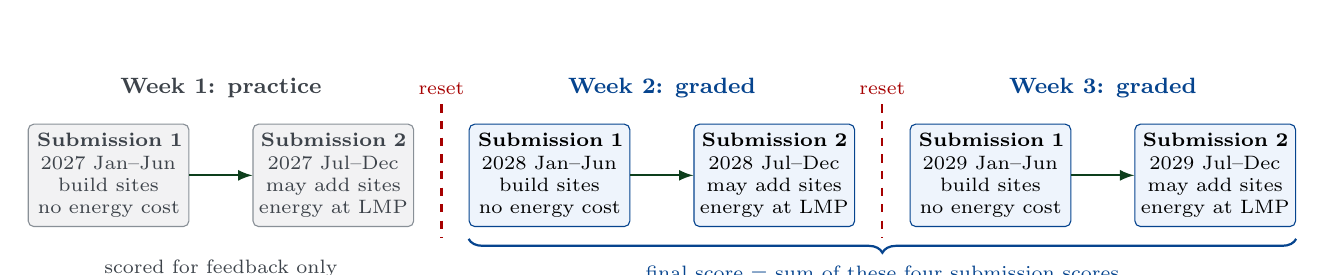
\begin{tikzpicture}[font=\scriptsize, >=latex,
  sub/.style={draw, rounded corners=2pt, align=center, minimum height=13mm, text width=19mm, inner sep=2pt},
  practice/.style={sub, draw=gray!70, fill=gray!8, text=gray!70!black},
  graded/.style={sub, draw=blue!65!black, fill=blue!7},
  carry/.style={->, thick, draw=green!50!black},
  reset/.style={dashed, thick, draw=red!65!black}]
  \foreach \w/\yr/\x/\style in {1/2027/0/practice, 2/2028/5.6/graded, 3/2029/11.2/graded} {
    \node[\style] (s1w\w) at (\x,0) {{\bfseries Submission 1}\\\yr{} Jan--Jun\\build sites\\no energy cost};
    \node[\style, right=8mm of s1w\w] (s2w\w) {{\bfseries Submission 2}\\\yr{} Jul--Dec\\may add sites\\energy at LMP};
    \draw[carry] (s1w\w.east) -- (s2w\w.west);
  }
  \node[above=2mm of $(s1w1.north)!0.5!(s2w1.north)$, font=\footnotesize\bfseries, text=gray!70!black] {Week 1: practice};
  \node[above=2mm of $(s1w2.north)!0.5!(s2w2.north)$, font=\footnotesize\bfseries, text=blue!65!black] {Week 2: graded};
  \node[above=2mm of $(s1w3.north)!0.5!(s2w3.north)$, font=\footnotesize\bfseries, text=blue!65!black] {Week 3: graded};
  \foreach \a/\b in {1/2, 2/3} {
    \coordinate (r\a) at ($(s2w\a.east)!0.5!(s1w\b.west)$);
    \draw[reset] ($(r\a)+(0,0.9)$) -- ($(r\a)+(0,-0.8)$);
    \node[font=\scriptsize, text=red!65!black, align=center, above] at ($(r\a)+(0,0.9)$) {reset};
  }
  \draw[decorate, decoration={brace, mirror, amplitude=5pt}, thick, blue!65!black]
    ($(s1w2.south west)+(0,-0.15)$) -- ($(s2w3.south east)+(0,-0.15)$)
    node[midway, below=6pt, text=blue!65!black] {final score = sum of these four submission scores};
  \node[below=3mm of $(s1w1.south)!0.5!(s2w1.south)$, font=\scriptsize, text=gray!70!black] {scored for feedback only};
\end{tikzpicture}

  \caption{The submission timeline. Arrows: the load connected in Submission 1
  becomes part of the base load for Submission 2 of the same week. Everything is
  removed between weeks.}
  \label{fig:timeline}
\end{figure}

\paragraph{Within a week.}
\begin{itemize}[leftmargin=*]
  \item Submission 1 connects sites to the grid with the representative base
    load.
  \item In Submission 2, the load that every team connected in Submission 1
    is \alert{part of the base load}: it is already on the grid and is not
    re-evaluated. You submit \alert{only new sites}, and they compete for the
    room that is left.
  \item Each site is scored once, in the submission where it is built, for its
    ten-year value.
  \item Everything \alert{resets} at the start of the next week, so you can
    improve your strategy based on what you saw the week before.
\end{itemize}

\paragraph{Time model.} Every submission uses the same \alert{representative
data for the next ten years}: five typical days of 24 hourly periods, 120
periods in all. Each day stands for a number of days of the year (the peak-load
day stands for one), so together the five days make up one typical year. We
assume that each of the next ten years looks like this typical year: the same
loads, the same network, and the same generators. A site, once connected, runs
for all ten years. Batteries
follow a daily cycle: they start each day half full and must end it half full.
The grid operator decides how your generator and battery run in every period,
and they can serve only your own load (\cref{sec:game,sec:model}).

\paragraph{Submission format.} One CSV per team with exactly this header
and one row per site:
\begin{lstlisting}[style=csvfile]
team_id,site_id,bus_id,connection_capacity_mw,generator_capacity_mw,storage_power_mw,storage_energy_mwh
\end{lstlisting}
\begin{itemize}[leftmargin=*]
  \item One \code{team_id} on every row; every \code{site_id} unique; every
    \code{bus_id} must exist in the representative data package.
  \item \alert{4 Capacities:} Connection capacity $C \ge 0$, generator capacity
    $0 \le G \le 0.5\,C$, and storage either $P = B = 0$ or $B = 4P$.
    A generator may run at most \alert{2 hours a day} at full output
    ($2G$ MWh per representative day), a stand-in for the run-hour limits in
    air permits for on-site engines~\cite{ecfr6366640,georgia2025permit}.
  \item In Submission 2, list \alert{only new sites}. Reusing a
    \code{site_id} of your Submission 1 makes the whole file invalid.
  \item File name: follow the format \alert{team\{x\}\_week\{x\}\_sub\{x\}.csv}, e.g., team07\_week2\_sub1.csv. Upload to: \alert{BrightSpace}.
\end{itemize}
Details and examples are in \cref{sec:csv}.

\paragraph{Validity.} Run \code{ercot-game-check-csv} with
\code{--artifact-dir} on the file you upload. \alert{A file that fails
validation scores 0} for that submission.

\newpage
% ---------------------------------------------------------------------------
\assignsection{Scoring and evaluation}{asg:scoring}

\paragraph{Score of one submission} (in US dollars):
\[
\begin{aligned}
  \text{score} = \text{IT value} &- \text{energy cost} - \text{generator operating cost}\\
  &- \text{generator capital} - \text{storage capital} - \text{site cost}.
\end{aligned}
\]

\begin{center}
\small
\begin{tabularx}{\linewidth}{@{}l X X@{}}
\toprule
Term & Value & How it is charged\\
\midrule
IT value & \$1,000 per MWh & Paid for every MWh of your load \alert{that is actually served}, over ten years.\\
Energy cost & \alert{L}ocational \alert{M}arginal \alert{P}rice (LMP) at your site & Grid purchases times the LMP, over ten years. \alert{Week 3 only; Weeks 1 and 2 have no energy cost.}\\
Generator operating cost & \$80 / \$150 / \$250 per MWh & Piecewise: first 25\% of capacity at \$80, next 50\% at \$150, last 25\% at \$250, over ten years.\\
Generator capital & \$2.0M per MW & On generator capacity, once, when it is built.\\
Generator run hours & 2 h per day & Each representative day, a generator of $G$\MW{} may produce at most $2G$\MWh{}.\\
Storage capital & \$400k per MW + \$250k per MWh & Once, when it is built. A 4-hour battery costs \$1.4M per MW of power.\\
Site cost & \$25M per MW & On connection capacity, once, when the site is built.\\
\bottomrule
\label{tab:hyperparameters}
\end{tabularx}
\end{center}
\alert{Ten years, in present value.} Each representative hour is weighted by
the number of days its day stands for, so the 120 hours make up one year of
8{,}760 hours, and ten such years make $87{,}600$ hours. All money in the score
is a \alert{present value}: a dollar earned in year $y$ counts as
$1/1.07^{y}$ dollars today (a 7\% discount rate, the rate U.S.\ federal
guidance long used for returns on private capital~\cite{omb2003circulara4}),
because money later is worth less than money now. Over ten years this multiplies every per-MWh amount by
$\frac{1}{10}\sum_{y=1}^{10} 1.07^{-y} = 0.702$. So one MW served in every hour
for ten years earns $87{,}600 \times \$1{,}000 = \$87.6$M, which is
\alert{\$61.5M in present value}. Energy and generator fuel are discounted the
same way. Capital is paid once, up front, so it is not discounted.
\Cref{sec:data} gives the formula. The scoring-rules file
\code{data/teaching/dispatch_scoring_rules_representative_v1.json} is the source
of these numbers.

\paragraph{Final score.} Your final score is the \alert{sum of your four
submission scores in Weeks 2 and 3}. 

\paragraph{One joint evaluation.} All valid plans are dispatched together in one
DCOPF per operating period, so whether your load is served depends on where
the other teams build. If the combined plan does not fit the grid:
\begin{itemize}[leftmargin=*]
  \item every team is served up to a \alert{common MW level}, and a team that
    asked for less is served in full;
  \item teams that can still grow keep rising until they are blocked;
  \item a team that would be served \alert{less than half} of its request
    gets \alert{nothing}.
\end{itemize}
\alert{Capital is always charged on what you \emph{requested}, served or not.} The rule
is explained in \cref{sec:projection} and specified in \cref{app:projection}.

\paragraph{What you get back.} After each submission: your score breakdown,
every team's service fraction, whether the projection was triggered,
and an interactive grid map with the total connection capacity per bus
(\cref{sec:results}). Other teams never see your individual plan.

\paragraph{Preview versus official score.} \code{ercot-game-preview} gives an
approximate score for your plan alone. Only the official evaluator, run by the
instructor with every team's plan, produces your score.

\newpage
% ---------------------------------------------------------------------------
\assignsection{Deliverables, grading, and conduct}{asg:conduct}

\paragraph{What you will learn.} By the end of the game you should be able to
\begin{itemize}[leftmargin=*]
  \item formulate a power-system planning decision as an optimization problem
    and solve it with an optimization package (DCOPF, hosting capacity);
  \item read locational marginal prices and congestion as signals for where
    new load can connect;
  \item size distributed generation and storage against network limits and
    energy prices;
  \item reason about a planning decision whose outcome depends on what other
    players do, as in an electricity market;
  \item use computational tools, including AI assistants, critically and
    reproducibly.
\end{itemize}

\paragraph{Deliverables.} The six CSV files, one per submission, uploaded by the
deadlines in \nameref{asg:glance}, and at the end a short presentation (tentatively scheduled for the \alert{last week}) and a
report explaining what your team did and why.

\paragraph{Grading.} The assignment counts for \alert{40 points} of the final
grade:
\begin{itemize}[leftmargin=*]
  \item \alert{30 points} for the presentation, the report, and your work;
  \item \alert{10 points} for your final game score $S$, the sum of your four
    graded submissions:
    \begin{itemize}
      \item \alert{5 absolute points}: $5 \times \min\!\big(1, \max(0, S/(2B))\big)$,
        where $B$ is the score of a simple reference plan published before Week
        2. These points do not depend on other teams, so everyone can earn all
        of them, and nobody gains by hurting another team.
      \item \alert{5 rank points}, by your rank among all teams:
    \end{itemize}
\end{itemize}
\begin{center}
\small
\begin{tabular}{@{}lccccc@{}}
\toprule
Rank & Top 20\% & 20--40\% & 40--60\% & 60--80\% & Bottom 20\%\\
Points & 5 & 4 & 3 & 2 & 1\\
\bottomrule
\end{tabular}
\end{center}
\alert{Bonus, up to 5 points:}
\begin{itemize}[leftmargin=*]
  \item \alert{Top three final scores}: 3, 2, and 1 points.
  \item \alert{Prediction or insight}, up to 2 points: the most accurate
    prediction of your own service fraction, stated with your Week 3
    Submission 1, or the best explanation in your presentation of why something
    happened in the game.
\end{itemize}
Week 1 is practice and earns no points.

\paragraph{Late and invalid submissions.} \alert{Late submission will not be accepted}, sinceall teams are evaluated together, and a late file cannot be added to a round that has
already been run. A late submission is treated as \alert{a zero}.

\paragraph{Working with other teams.} \alert{Teams may talk to or
coordinate with each other}. In any case, do not share your CSV, your exact
plan, or shared chat links that contain it with another team.

\paragraph{Use of AI.} You may use AI tools for any part of this assignment
(\cref{sec:ai}). Your team is responsible for every number you submit and
must be able to explain its plan. Do not paste passwords, tokens, or other
teams' information into an AI tool.

\paragraph{Academic integrity.} Purdue's academic integrity policy applies.
Each team's plans must be its own work.

\paragraph{Problems with your results.} If you think your submission was
evaluated incorrectly, contact \alert{Minghao} via \alert{mmou@purdue.edu} within \alert{7} days of the
results release.

\newpage
\phantomsection\addcontentsline{toc}{part}{Part II: The Tutorial}
\begin{center}
\Large\bfseries Part II: The Tutorial
\end{center}

\begin{keybox}[Quick start]
\begin{enumerate}[leftmargin=*]
  \item Read Part I, the assignment (\nameref{asg:glance} to
    \nameref{asg:conduct}).
  \item Set up the GitHub repository (\cref{sec:setup}).
  \item Try the AI-agent walkthrough on the IEEE 14-bus demo (\cref{sec:agent}).
  \item Read \cref{sec:game,sec:score} so you know what earns points.
  \item Explore the representative data (\cref{sec:data}).
  \item Write your plan as a CSV and run the checker on it (\cref{sec:csv}).
  \item Preview the plan, change one thing at a time, and repeat (\cref{sec:preview,sec:strategy}).
  \item Go through the checklist in \cref{sec:checklist} and submit.
  \item When the results come out, read them as described in \cref{sec:results}.
\end{enumerate}
\end{keybox}

\begingroup
\setlength{\parskip}{0pt}
% \setcounter{tocdepth}{1}
\tableofcontents
\endgroup
\newpage

This part walks you through the assignment from start to finish: what the
game is, how your plan is scored, how to explore the data, how to write and
check your submission, and how to use AI tools along the way. The numbers come
from the scoring-rules files in \code{data/teaching/}, and
\code{docs/HYPERPARAMETERS.md} lists every game parameter with its source.

% ---------------------------------------------------------------------------
\section{The game in one page}\label{sec:game}

Your team is a data-center operator. You choose \alert{where} to connect computing
load to a public-data-informed planning model of the Texas grid, \alert{how large (in MW)} connection is, and whether to build your own \alert{generation} and \alert{battery storage} collocated with it. The instructor, acting as the grid operator, then runs one DCOPF dispatch with every team's plan in it, and scores each team. The grid is the public ACTIVSg2000 test
system~\cite{activsg2000}: 2,000 buses, 3,206 branches, and 544 generators,
stored in the MATPOWER case format~\cite{matpower}.

\subsection{What you decide}
Your plan is a list of \emph{sites}. For each site you choose four numbers:

\begin{center}
\small
\begin{tabularx}{\linewidth}{@{}l l X@{}}
\toprule
Decision & Unit & Meaning\\
\midrule
Bus & -- & Where the site connects to the network (a \code{bus_id}).\\
Connection capacity $C$ & MW & Your requested computing \alert{load cap} at this site. \\
Generator capacity $G$ & MW & Optional private generator at the site, at most $0.5\,C$.\\
Storage power $P$ / energy $B$ & MW / MWh & Optional battery: either both zero, or $B = 4P$.\\
\bottomrule
\end{tabularx}
\end{center}

\alert{You only choose sites and four capacities.} The grid operator decides how your
generator and battery run in each operating period. Your generator and battery serve only
your own load: they never export to the grid or to another team.

\subsection{Schedule and data}
The schedule and the timeline are set out in \nameref{asg:rules}
(\cref{fig:timeline}). In short: three weeks, each playing the same ten-year
game in two submissions; Week 1 is practice, Weeks 2 and 3 count, and only
Week 3 charges energy.

Every submission uses the same \alert{representative data for the next ten
years}, in \code{data/processed/activsg2000_representative_v1/}: five typical
days of 24 hourly periods, 120 periods in all. They were picked from a year of
hourly load data: four days that each stand for a group of similar days, plus
the peak-load day, which stands for itself.
\begin{center}
\small
\begin{tabular}{@{}lcccc@{}}
\toprule
Day & Periods & Stands for (days per year) & Daily energy (GWh) & Peak (GW)\\
\midrule
1 (winter) & 0--23 & 83.77 & 1{,}569 & 69.4\\
2 (spring) & 24--47 & 99.73 & 1{,}493 & 66.2\\
3 (summer) & 48--71 & 82.77 & 1{,}653 & 72.9\\
4 (late summer) & 72--95 & 97.73 & 1{,}729 & 76.1\\
5 (peak-load day) & 96--119 & 1 & 1{,}780 & 78.2\\
\bottomrule
\end{tabular}
\end{center}
The days sum to 365. Your CSV uses one row per connection site; the evaluator
applies that plan to all 120 periods.

\begin{keybox}[From 120 hours to ten years]
Period $t$ belongs to a day that stands for $d_t$ days of the year, so it
stands for $d_t$ hours of each year ($\sum_t d_t = 8{,}760$) and $10\,d_t$ hours
of the ten years ($87{,}600$ in all). Every per-MWh amount (IT value, energy,
generator fuel) earned in period $t$ is counted in present value:
\[
  \text{value} = \sum_t (\text{\$ per hour in period } t) \times d_t \times A,
  \qquad
  A = \sum_{y=1}^{10} \frac{1}{1.07^{y}} = 7.02,
\]
where $A$ adds up the ten years, each discounted at 7\% per year. Since
$A = 0.702 \times 10$, a present value is $0.702$ times the plain ten-year total.
For one MW served in every hour: $87{,}600 \times \$1{,}000 \times 0.702 =
\$61.5$M. (The rules file stores the weights $d_t A$ for each period.)
Capital is paid once, up front, and is not discounted. With \code{daily\_exact\_cycle}, a battery starts each
representative day at $B/2$ and must end it at exactly $B/2$.
\end{keybox}

\begin{keybox}
In Submission 2, the load that all teams connected in Submission 1 is part of
the base load. A site added in Submission 2 earns the same ten-year value as
one built in Submission 1, but it competes only for the room that is left.
\end{keybox}

\begin{figure}[htbp]
  \centering
  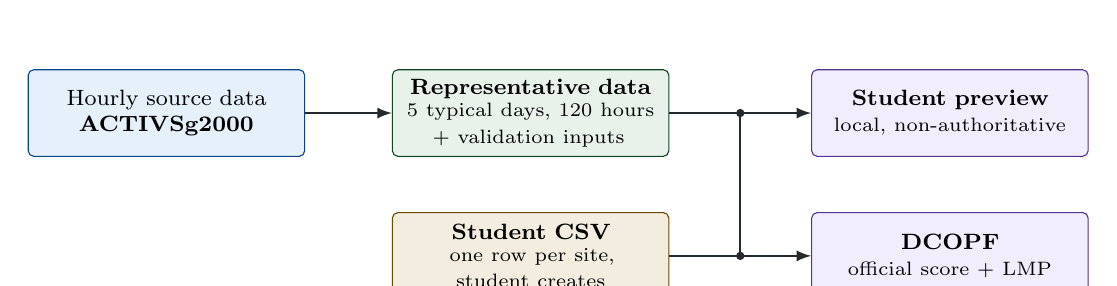
\begin{tikzpicture}[font=\footnotesize, >=latex, node distance=7mm and 11mm]
  % Semantic source anchors: ACTIVSg2000 hourly source, representative-day release, student CSV, daily-cycle dispatch, and scores.
  \tikzset{artifact/.style={draw, rounded corners=2pt, align=center, minimum height=11mm, text width=33mm, inner sep=3pt, execute at begin node={\hyphenpenalty=10000 }},
    source/.style={artifact, fill=blue!10, draw=blue!65!black},
    release/.style={artifact, fill=green!10, draw=green!55!black},
    submission/.style={artifact, fill=orange!12, draw=orange!70!black},
    outcome/.style={artifact, fill=purple!10, draw=purple!65!black},
    flow/.style={->, thick, draw=ink},
    junction/.style={circle, fill=ink, inner sep=0pt, minimum size=3pt}}
  \node[source] (public) {Hourly source data\\{\bfseries ACTIVSg2000}};
  \node[release, right=of public] (package) {{\bfseries Representative data}\\{\scriptsize 5 typical days, 120 hours\\+ validation inputs}};
  \node[submission, below=of package] (csv) {{\bfseries Student CSV}\\{\scriptsize one row per site,\\student creates}};
  % Vertical bus: both inputs reach both evaluators without crossing a box.
  \coordinate (bus) at ([xshift=9mm]package.east);
  \node[outcome, anchor=west] (preview) at ([xshift=9mm]bus |- package) {{\bfseries Student preview}\\{\scriptsize local, non-authoritative}};
  \node[outcome, anchor=west] (eval) at ([xshift=9mm]bus |- csv) {{\bfseries DCOPF}\\{\scriptsize official score + LMP}};
  \draw[flow] (public) -- (package);
  \draw[thick, draw=ink] (package.east) -- (bus |- package) -- (bus |- csv);
  \draw[thick, draw=ink] (csv.east) -- (bus |- csv);
  \draw[flow] (bus |- package) -- (preview.west);
  \draw[flow] (bus |- csv) -- (eval.west);
  \node[junction] at (bus |- package) {};
  \node[junction] at (bus |- csv) {};
\end{tikzpicture}

  \caption{What you receive and what you submit. The released package gives
  you the network plus scenario context and validation inputs. You create the
  plan (CSV submission), and can preview it yourself, but only the official evaluator
  produces your score.}
  \label{fig:pipeline}
\end{figure}

% ---------------------------------------------------------------------------
\section{How your score is computed}\label{sec:score}

For each submission, your score in US dollars is
\[
\begin{aligned}
  \text{score} = \text{IT value}
  &- \text{energy cost} - \text{generator operating cost}\\
  &- \text{generator capital} - \text{storage capital} - \text{site cost}.
\end{aligned}
\]
The coefficients are in the table in \nameref{asg:scoring}: IT value
\$1,000/MWh served, energy at the LMP in Week 3 only, a generator curve of
\$80/\$150/\$250 per MWh, all over ten years, and capital of \$25M/MW for a
site, \$2.0M/MW for a generator (which may produce at most two hours' worth
of its capacity per day), and \$400k/MW plus \$250k/MWh for storage,
charged once when built.
Storage has no operating cost. This section shows what those numbers mean for
a plan.

\subsection{A worked example}\label{subsec:worked_example}
Suppose you build one 50\MW{} site and nothing else, and all of its load is
served in every period. Baseline LMPs are about \$18/MWh.

\textbf{In Week 1 or Week 2} (no energy cost):
\begin{align*}
  \text{IT value}  &= 50 \times 87{,}600 \times 1{,}000 \times 0.702 = \$3{,}076.3\text{M}\\
  \text{site cost} &= 50 \times 25\text{M} = \$1{,}250.0\text{M}\\
  \text{score}     &= \$1{,}826.3\text{M}
\end{align*}

\textbf{In Week 3} (energy at the LMP):
\begin{align*}
  \text{energy cost} &\approx 50 \times 87{,}600 \times 18 \times 0.702 = \$55.4\text{M}\\
  \text{score}       &\approx \$1{,}770.9\text{M}
\end{align*}

Each served MW earns about \$61.5M (present value) over ten years against a one-time site cost
of \$25M, so a site breaks even once about \alert{41\% of its load is served}.

\begin{keybox}
Energy is cheap compared with the value of serving load (\$18 against
\$1,000 per MWh). What decides your score is \alert{whether the grid can
actually deliver power to your site.} Load the network cannot serve still pays
the full site cost.
\end{keybox}

\begin{exercisebox}
A team adds a 30\MW{} site in Submission 2 of Week 3, and it is fully served
at an LMP of about \$18/MWh. Estimate its score. \emph{(Answer:
$30 \times 87{,}600 \times (1{,}000 - 18) \times 0.702 - 750\text{M} \approx \$1{,}063\text{M}$.)}
\end{exercisebox}

\subsection{You are not the only player}\label{sec:projection}
The worked example in Section \ref{subsec:worked_example} quietly assumed that \alert{all of your load is served.} Whether it is depends on more than your own plan. Every team reads the same rules and does
the same arithmetic, so every team is tempted by the same plan: build big,
build early, and pick buses (sites) where the network looks strong. Each of those plans
can be fine on its own, and your preview, which runs without the other teams,
will say so. But \alert{the spare capacity of the grid is shared}. If too many teams
crowd the same part of the network, the combined plan has no feasible dispatch,
even though no single plan caused the problem.

\begin{quote}
\itshape ``The hard thing in life is getting you to come out of your own selves
a bit, realizing it's `not all about you.'\,''
\end{quote}

When the combined plan of all teams is infeasible, the evaluator has to decide who gets
served. It applies a \alert{fair
projection} based on the \emph{uniform rule}:
\begin{enumerate}[leftmargin=*]
  \item \alert{Service fractions.} Each team $i$ gets a single fraction
    $\alpha_i \in [0,1]$ that scales the connection capacities of all its
    sites in every period.
  \item \alert{Equal level.} A common level $t$ (in MW) rises from zero, and
    team $i$ is served $\min(r_i, t)$, where $r_i$ is its total requested
    connection capacity. The level stops at the largest $t$ for which the
    joint dispatch is feasible in every operating period. A team that asked
    for less than $t$ is served in full.
  \item \alert{Fill the slack.} If some teams can still grow without hurting
    a team that is already stuck, their level keeps rising until every team is
    either fully served or blocked.
  \item \alert{Minimum allocation.} A team that would be served less than
    \alert{50\%} of its request gets \alert{nothing}. The largest such request
    is dropped first, and the allocation is recomputed for the rest.
\end{enumerate}

This changes the question you should ask. Your served load, and so
whether you clear the break-even points above, depends on what everyone else
builds. A bigger request does not buy you priority: you are never served more
than the common level, and a request so large that it would be served less than
half is dropped entirely, while capital is still charged on the full
capacity you submitted. So the question is not only ``how much load can my
site take?'' but also ``how much room will be left for me once the other teams
have built, and what do they expect me to do?''

\Cref{sec:twoteam} works through a stylized two-team example at two
neighboring buses.

\begin{exercisebox}[Think about it]
Suppose you expect most teams to crowd the best-connected buses. What do you
gain and what do you risk by choosing a less popular location instead? What
would the Week 1 results tell you about how other teams actually behave?
\end{exercisebox}

% ---------------------------------------------------------------------------
\section{How the grid operator runs your plan}\label{sec:model}

The evaluator solves a DCOPF on the ACTIVSg2000 network for each of the 120
representative hours, with all teams' sites added. The existing network,
generators, and base loads come from the representative data package (in
Submission 2, the base load also contains the Submission 1 sites). \Cref{fig:site}
shows what one row of your CSV adds at a bus $k$.

\begin{figure}[htbp]
  \centering
  \begin{tikzpicture}[font=\footnotesize, >=latex]
  % Semantic anchors: ACTIVSg2000, student CSV, DCOPF, student preview.
  % One student CSV row attaches a site (load, private generator, storage) to one network bus.
  \tikzset{part/.style={draw, rounded corners=2pt, align=center, minimum height=10mm, text width=40mm, inner sep=3pt,
      execute at begin node={\hyphenpenalty=10000 }},
    load/.style={part, fill=orange!12, draw=orange!70!black},
    gen/.style={part, fill=green!10, draw=green!55!black},
    store/.style={part, fill=purple!10, draw=purple!65!black},
    grid/.style={draw=blue!65!black, fill=blue!10, rounded corners=6pt, align=center, minimum height=34mm, text width=27mm,
      execute at begin node={\hyphenpenalty=10000 }},
    link/.style={thick, draw=ink}}
  \node[grid] (net) at (0,0) {{\bfseries ACTIVSg2000}\\{\bfseries network}\\[3pt]hourly DCOPF with all teams' sites};
  \node[circle, draw=blue!65!black, fill=white, thick, minimum size=10mm, align=center] (bus) at (5.0,0) {bus $k$};
  \node[gen] (g) at (10.2,0) {{\bfseries Private generator}\\$0\le g_t\le G$, $\le 2G$ MWh/day\\\$80/150/250 per MWh};
  \node[load, above=3mm of g] (it) {{\bfseries IT load} $\alpha C$\\earns \$1,000 per MWh served};
  \node[store, below=3mm of g] (s) {{\bfseries Storage} $-P\le p_t\le P$\\$B=4P$, no operating cost};
  \begin{scope}[on background layer]
    \node[draw=orange!70!black, dashed, rounded corners=4pt, fit=(it)(g)(s), inner sep=5pt,
      label={[font=\scriptsize\bfseries, text=orange!70!black]above:your site = one row of the student CSV}] (site) {};
  \end{scope}
  \draw[link] (net.east) -- node[above=1pt, font=\scriptsize] {grid purchase} node[below=1pt, font=\scriptsize] {paid at LMP $\lambda_{k,t}$} (bus.west);
  \coordinate (tap) at ($(g.west)+(-7mm,0)$);
  \draw[link] (bus.east) -- (tap);
  \draw[link] (tap |- it) -- (tap |- s);
  \draw[link, ->] (tap |- it) -- (it.west);
  \draw[link, <-] (tap) -- (g.west);
  \draw[link, <->] (tap |- s) -- (s.west);
\end{tikzpicture}

  \caption{One site in the dispatch. The site draws $\alpha C$ of IT load; your
  generator and battery can cover part of it, and the rest is bought from the
  grid at the bus LMP.}
  \label{fig:site}
\end{figure}

For a site at bus $k$ in period $t$, the evaluator adds:
\begin{itemize}[leftmargin=*]
  \item a fixed load $\alpha C$ (normally $\alpha \in [0,1]$, cf. Section~\ref{sec:projection});
  \item a private generator $0 \le g_t \le G$ with the piecewise cost in \nameref{asg:scoring};
  \item a battery with signed power $p_t$ (positive = discharge), limited by
    $-P \le p_t \le P$.
\end{itemize}
Your grid purchase rate in period $t$ is $\alpha C - g_t - p_t$. The generator and
battery can only cover your own team's load at that bus; they cannot push power
back into the grid.

\subsection{Storage}
Each battery follows the model below, with hourly steps and 100\% efficiency.
The signed variable $p_{d,h}$ is a power rate in MW: positive means discharge
and negative means charge. Let $\Delta t=1$ hour.
\begin{gather*}
  e_{d,h} = e_{d,h-1} - \Delta t\,p_{d,h}, \qquad 0 \le e_{d,h} \le B, \qquad -P \le p_{d,h} \le P, \qquad \Delta t\,p_{d,h} \le e_{d,h-1},\\
  e_{d,0} = 0.5B, \qquad e_{d,24} = 0.5B \qquad \text{for each representative day }d.
\end{gather*}
The battery starts every representative day half full and must end it at
exactly half full after 24 hours (\cref{fig:soc}). There is no state-of-charge
carryover from one day to the next. Discharge at a bus cannot exceed your own
load there.

\begin{figure}[htbp]
  \centering
  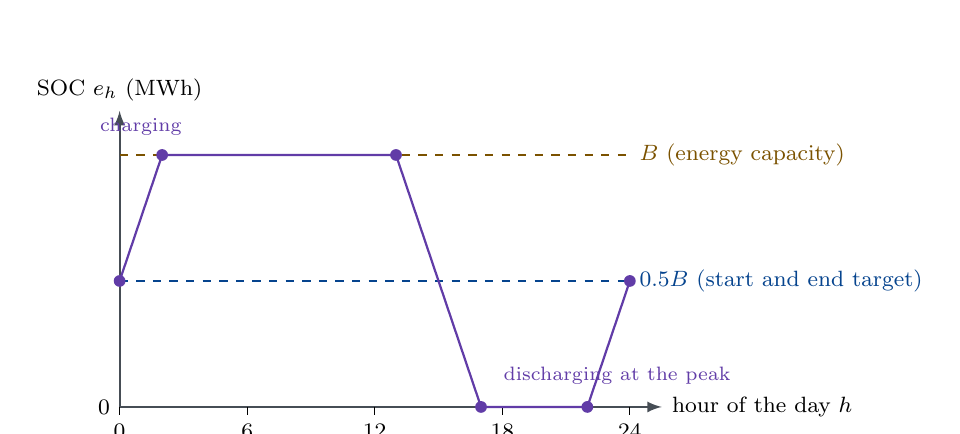
\begin{tikzpicture}[font=\footnotesize, >=latex, x=0.27cm, y=0.8cm]
  % Illustrative hourly SOC path over one representative day with B = 4P:
  % starts and ends exactly at 0.5B, moves by at most P MWh per hour.
  \tikzset{axis/.style={->, thick, draw=gray!80!black},
    point/.style={circle, fill=purple!75!black, inner sep=1.5pt}}
  \draw[axis] (0,0) -- (25.5,0) node[right] {hour of the day $h$};
  \draw[axis] (0,0) -- (0,4.7) node[above] {SOC $e_h$ (MWh)};
  \foreach \h in {0,6,12,18,24} {\draw (\h,0) -- (\h,-0.12) node[below] {\h};}
  \draw[dashed, orange!80!black] (0,4) -- (24,4) node[right] {$B$ (energy capacity)};
  \draw[dashed, blue!65!black] (0,2) -- (24,2) node[right] {$0.5B$ (start and end target)};
  \node[left] at (0,0) {$0$};
  \draw[thick, purple!75!black] (0,2) -- (2,4) -- (13,4) -- (17,0) -- (22,0) -- (24,2);
  \foreach \x/\y in {0/2,2/4,13/4,17/0,22/0,24/2} {\node[point] at (\x,\y) {};}
  \node[font=\scriptsize, text=purple!75!black, align=center] at (1,4.45) {charging};
  \node[font=\scriptsize, text=purple!75!black, anchor=west] at (17.6,0.5) {discharging at the peak};
\end{tikzpicture}

  \caption{An illustrative one-day battery schedule with $B = 4P$: it starts
  at $0.5B$, stays between $0$ and $B$, moves by at most $P$ MWh per hour, and
  returns to exactly $0.5B$ at the end of the day. The evaluator chooses this
  schedule independently for each representative day.}
  \label{fig:soc}
\end{figure}

\subsection{Prices}
The LMP at your bus is the dual of that bus's power balance in the joint
dispatch, clipped at zero. In Week 3, energy is settled against LMPs computed
from the actual joint dispatch containing all accepted teams. Optional baseline LMP artifacts may be generated for
diagnostics. With teams' load added,
lines can congest and the LMP at your bus can rise.

\begin{exercisebox}
A battery has $P = 5\MW$ and $B = 20\MWh$. It starts a representative day at
the required state of charge. Can it discharge at 5\MW{} for two hours in a
row? What is the state of charge after each hour? \emph{(Answer: it starts at
10\MWh, is at 5\MWh{} after one hour and 0\MWh{} after two; it cannot
discharge in a third hour until it has charged. It must also return to exactly
10\MWh{} by the end of the day.)}
\end{exercisebox}

% ---------------------------------------------------------------------------
\section{Set up your computer}\label{sec:setup}

You need Python 3.11 or newer and the course repository. From a terminal:
\begin{lstlisting}[language=bash]
git clone <course-repository-URL> ercot-game
cd ercot-game
python3 -m venv .venv
source .venv/bin/activate        # Windows: .venv\Scripts\activate
python -m pip install -e ".[tutorial]" pandas
\end{lstlisting}

\alert{Run every command in this tutorial from the repository root with the virtual
environment active.} Check the installation by validating the example
submission (\cref{sec:csv} explains the output):
\begin{lstlisting}[language=bash]
ercot-game-check-csv --file examples/eight_team_round/submissions/team-01.csv
\end{lstlisting}

The files you will use most:

\begin{center}
\begin{tabularx}{\linewidth}{@{}l X@{}}
\toprule
Path & What it is\\
\midrule
\code{docs/HYPERPARAMETERS.md} & Every game parameter, with its value and source.\\
\code{data/processed/activsg2000_representative_v1/} & Representative data: five typical days, 120 hourly periods.\\
\code{data/teaching/dispatch_scoring_rules_representative_v1.json} & Scoring coefficients and the ten-year weights used by the preview and the evaluator.\\
\code{ercot-game-check-csv} & Checker for your CSV (also \code{scripts/check_submission.py}).\\
\code{ercot-game-preview} & Approximate scoring run for your plan.\\
\code{docs/student_tutorial/notebooks/} & Small companion notebooks (see below).\\
\bottomrule
\end{tabularx}
\end{center}

The notebooks in \code{docs/student_tutorial/notebooks/} use tiny made-up
fixtures, not the real data. They are useful for seeing the mechanics in
isolation: \code{03_three_bus_dcopf.ipynb} solves a three-bus DCOPF with the
same solver the evaluator uses, \code{04_storage_soc.ipynb} traces a battery's
state of charge, and \code{05_csv_validation.ipynb} calls the checker from
Python.

% ---------------------------------------------------------------------------
\section{Using AI for this assignment}\label{sec:ai}

\alert{You are encouraged to use AI tools} such as ChatGPT, Claude, Gemini, GitHub
Copilot, Claude Code, or Codex. You are still responsible for every number you
submit and must be able to explain your plan. This section is for anyone who
has not used these tools much. If you are already familiar with AI tools, you can skip this section.

\subsection{Which kind of tool}
\begin{itemize}[leftmargin=*]
  \item \textbf{Chat assistants} (ChatGPT, Claude, Gemini in a browser) are best
    for explaining concepts, writing short scripts, and decoding error
    messages. They only see what you paste in. Most of them can be used for free. However, without subscriptions, we may be limited to only the use of basic models.
  \item \textbf{Coding assistants/AI agents} \alert{[recommended]} (Claude Code, Codex, Copilot in your editor)
    can read the GitHub repository and run commands for you. They are faster once you
    are comfortable, but check what they change. Most of them require subscriptions. \alert{All the demos in the tutorials used coding assistants, since it is not easy for char assistants to manipulate local files.}\footnote{There are in fact some advanced tools that allow chat assistants to get access to and manipulate local files. You can search for those tools online. However, using those tools comes with risks of getting your account suspended.}
\end{itemize}
If you are new to this, start with a chat assistant and copy code into your
own files. Each tool has an official getting-started guide:

\begin{center}
\small
\begin{tabularx}{\linewidth}{@{}l l X@{}}
\toprule
Tool & Kind & Getting started\\
\midrule
ChatGPT & Chat & \href{https://help.openai.com/en/articles/12677804-what-is-chatgpt-faq}{What is ChatGPT: FAQ}\\
Claude & Chat & \href{https://support.claude.com/en/articles/8114491-get-started-with-claude}{Get started with Claude}\\
Gemini & Chat & \href{https://support.google.com/gemini/answer/13275745}{Use Gemini Apps}\\
GitHub Copilot & Coding (editor) & \href{https://docs.github.com/en/copilot/get-started/quickstart-for-using-github-copilot-in-your-ide}{Quickstart for GitHub Copilot in your IDE}\\
Claude Code & Coding (terminal) & \href{https://code.claude.com/docs/en/quickstart}{Claude Code quickstart}\\
Codex & Coding (terminal) & \href{https://developers.openai.com/codex/cli}{Codex CLI}\\
\bottomrule
\end{tabularx}
\end{center}

GitHub Copilot is free for verified students, see
\href{https://docs.github.com/en/copilot/how-tos/copilot-on-github/set-up-copilot/enable-copilot/set-up-for-students}{Access GitHub Copilot for free as a student}.

\subsection{How to write a good prompt}
The AI knows DCOPF but knows nothing about this assignment. Give it four
things: 
\begin{itemize}
  \item the \textbf{goal},
  \item the \textbf{context} (paste file headers, a few rows, error messages),
  \item the \textbf{constraints}, 
  \item the \textbf{form} of answer you want.
\end{itemize}

\begin{promptbox}[Weak prompt]
Write code to analyze the data.
\end{promptbox}

\begin{promptbox}[Better prompt]
I am working in Python with pandas. I have a file \code{branch_limits.csv} with
columns \msg{branch_id, from_bus_id, to_bus_id, reactance_pu, thermal_limit_mva, status}.
Here are its first three rows: [paste]. Write code that, for each bus, adds
up \code{thermal_limit_mva} over in-service branches (\msg{status == 1})
connected to that bus, and prints the 20 buses with the largest total.
Explain each line briefly.
\end{promptbox}

\subsection{Work in a loop}
Treat the AI as a pair programmer. Ask for something small, run it, and paste
back exactly what happened, including the full error message. Repeat until it
works, then ask it to explain the final version so you understand it.

\begin{promptbox}
I ran your script and got this error:
\msg{KeyError: 'thermal_limit'}. The column names are exactly:
\code{branch_id,from_bus_id,to_bus_id,reactance_pu,thermal_limit_mva,status}.
Please fix the script.
\end{promptbox}

\begin{aibox}
The column is called \code{thermal_limit_mva}, not \code{thermal_limit}.
Change line 6 to \code{branches["thermal_limit_mva"]} and run it again.
\end{aibox}

\subsection{Check what the AI tells you}
\alert{AI tools are often confidently wrong about assignment-specific details (and this is the reason why you need to provide enough context to AI agents).} They
might invent a CSV column, assume you schedule the battery yourself, or use
made-up prices. Before you rely on an answer:
\begin{itemize}[leftmargin=*]
  \item \textbf{Run it.} Code that has not run is a guess.
  \item \textbf{Check the numbers} against this tutorial and the rules JSON.
  \item \textbf{Try a case you can do by hand}, such as the worked example in
    \cref{sec:score}.
  \item \textbf{Ask for its assumptions}: ``What did you assume that is not in
    the files I gave you?''
\end{itemize}

\subsection{Privacy}
\alert{Do not upload passwords, access tokens, or other credentials.} Your plan is
your team's competitive information, so do not share it with other teams,\footnote{However, it is possible to cooperate with other teams. It is also an interesting direction to explore.}
including through shared chat links. Public data from the repository is fine
to paste.

% ---------------------------------------------------------------------------
\section{Walk through the workflow with an AI agent}\label{sec:agent}

This section shows the whole workflow, from reading the rules to a joint
evaluation with a rival team, done by talking to an AI agent. It uses a
small \alert{IEEE 14-bus demo} that ships with the repository
(\code{data/teaching/ieee14_demo_representative}): 14 buses, 20 lines, 5
generators, and the same five representative days (120 hourly periods) and
ten-year scoring as the game. Every command runs in a few seconds, so you can
repeat the session yourself. The demo is for practice only: the game itself
runs on \texttt{ACTIVSg2000}, and the demo's numbers do not carry over.

\begin{figure}[htbp]
  \centering
  % Drawn by docs/guest_lecture/scripts/make_figures.py (workflow()); copied here.
  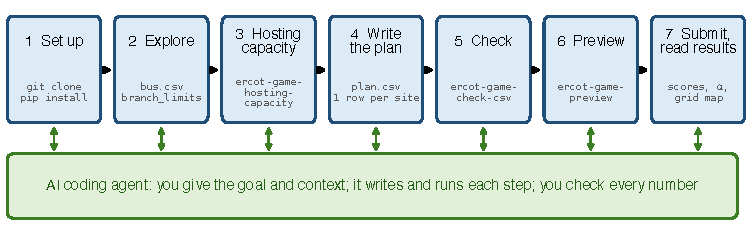
\includegraphics[width=\linewidth]{figures/workflow.pdf}
  \caption{The workflow in the repository, with an AI agent in the
  loop. Each step has its own section: set up (\cref{sec:setup}), explore
  (\cref{sec:data}), hosting capacity (\cref{sec:hc}), write and check the plan
  (\cref{sec:csv}), preview (\cref{sec:preview}), and read the results
  (\cref{sec:results}). The six prompts below walk through steps 2--7.}
  \label{fig:workflow}
\end{figure}

\paragraph{How the session was run.} A coding agent (Claude Opus 5.5) was started in a
fresh clone of the repository with the package installed (\cref{sec:setup}).
It had not seen the repository before. The six prompts below were typed one
after another in the same session. The replies are real
but shortened, with \msg{[...]} marks a cut. The complete prompts and replies are
in \code{docs/student_tutorial/ai_walkthrough/}. To start an agent yourself,
open a terminal in the repository folder and run, for example, \code{claude}
(Claude Code) or \code{codex} (Codex CLI).

Watch how each prompt is written. It states the \alert{goal}, names the
\alert{files and commands}, sets \alert{constraints} (``do not change any
files'', ``under 150 words''), and asks for the \alert{form} of the answer
(``a table'', ``show the commands''). After every reply, a box lists what you
should check yourself before you rely on it.

\subsection{Step 1: understand the assignment}
\begin{promptbox}[Prompt 1]
I just cloned this repository for my ECE 51032 course project. Read the README
and Part I of \code{docs/student_tutorial/main.tex} \alert{(context)}, then explain in under 150 words \alert{(constraint)}: what my team submits, how it is scored, and which commands I will use. \alert{(deliverables)}
Do not change any files \alert{(constraint)}.
\end{promptbox}
\begin{aibox}[Agent reply (shortened)]
\textbf{What you submit:} one CSV per submission, two a week for three weeks
(six files in all). [...] The rules are $G \le 0.5C$ and storage either zero or
$B = 4P$. Submission 2 lists only new sites. You also give a final presentation
and a report.

\textbf{Scoring:} score = IT value (\$1,000/MWh served, over 10 years) $-$
energy cost (charged at the LMP, Week 3 only) $-$ generator operating cost $-$
capital costs [...]. Your final score is the sum of the four Week 2 and 3
submissions. [...]

\textbf{Commands:} \code{ercot-game-check-csv} [...] and
\code{ercot-game-preview}. Note: the README describes an older six-hour setup
(\$6,500/MWh). Follow Part I.
\end{aibox}
\begin{warningbox}[Check it yourself]
The agent noticed that two documents disagree and said which one it trusted,
which is exactly what you want. But it left out a tool you will need,
\code{ercot-game-hosting-capacity}. Compare its summary with
\nameref{asg:rules} and \nameref{asg:scoring} rather than trusting a summary.
\end{warningbox}

\subsection{Step 2: look at the data}
\begin{promptbox}[Prompt 2]
We will practice on the small IEEE 14-bus demo package in
\code{data/teaching/ieee14_demo_representative} before touching the real grid.
Summarize it: number of buses, lines, and generators, total load, the number of
operating periods, and the five lines with the smallest thermal limits. Show
the commands you ran.
\end{promptbox}
\begin{aibox}[Agent reply (shortened)]
\textbf{Buses:} 14. \textbf{Lines:} 20, all in service. \textbf{Generators:} 5,
with 772.4\MW{} total capacity [...]. \textbf{Load:} the base load is
259.0\MW. Across the periods it ranges from 224.5 to 301.7\MW{} [...].
\textbf{Operating periods:} 120. That is 5 representative days of 24 one-hour
periods. The day weights add up to 365, and the peak day has a weight of 1.
\textbf{Five smallest thermal limits:} 12--13 (20 MVA), 10--11 (25), 13--14
(25), 6--11 (30), 6--12 (30). br16 (9--10) is also at 30 MVA, so the 4th and
5th places are a three-way tie at that limit.
\end{aibox}
\begin{warningbox}[Check it yourself]
Open \code{branch_limits.csv}: \alert{four} lines are at 30 MVA, not three.
The agent missed 9--14, which matters later because it is one of the lines
that limits buses 13 and 14. Small slips like this are common; spot-check any
table an agent gives you.
\end{warningbox}

\subsection{Step 3: hosting capacity}
\begin{promptbox}[Prompt 3]
Use \code{ercot-game-hosting-capacity} to compute the hosting capacity of every
bus in the demo package over all 120 hours. Give me a table of each bus's
minimum hosting capacity, sorted from largest to smallest, and say in one
sentence what this number means. Which two buses would you shortlist for a
data center, and why?
\end{promptbox}
\begin{aibox}[Agent reply (shortened)]
\begin{lstlisting}[language=bash]
ercot-game-hosting-capacity \
  --artifact-dir data/teaching/ieee14_demo_representative \
  --horizon 120 --period-count 120 --output-dir <tmp>/hc14
# backend highs, bus_count 14, completed_point_count 1680, failed_point_count 0, wall_time 1.6 s
\end{lstlisting}
The columns are in the order of \code{bus_ids} in the metadata file
(\code{1,10,11,...}), not numeric order, so I matched them up by that list.
\begin{center}
\small
\begin{tabular}{@{}lrrrrrrrrrrrrrr@{}}
\toprule
Bus & 1 & 2 & 5 & 4 & 3 & 7 & 8 & 6 & 9 & 13 & 11 & 10 & 12 & 14\\
Min HC (MW) & 471 & 429 & 311 & 241 & 180 & 178 & 178 & 169 & 103 & 51 & 45 & 45 & 43 & 38\\
\bottomrule
\end{tabular}
\end{center}
\textbf{What it means:} a bus's minimum hosting capacity is the most new load
you could add at that bus alone [...] that the grid can still serve in every
one of the 120 hours [...]. For every bus the lowest value falls in hour 109.
\textbf{Shortlist: buses 1 and 2.} [...] \textbf{One caution:} these numbers
are for one bus at a time, and they don't add up. Every team will see the same
table, so buses 1 and 2 may get crowded.
\end{aibox}
\begin{warningbox}[Check it yourself]
Re-run one bus yourself (add \code{--bus-id 14}) and compare. The agent caught
a real trap, the column order of the output file. Its caveat, that every team
sees the same table, is the most important line of the reply.
\end{warningbox}

\subsection{Step 4: write and check a plan}
\begin{promptbox}[Prompt 4]
Write a plan for team-demo with one site at each of the two buses you
shortlisted, each at about half of its hosting capacity, with no generator and
no battery. Save it as \code{runs/demo/plan.csv} and check it with
\code{ercot-game-check-csv} against the demo package. Then make a copy with a
mistake, a generator larger than its connection, and show me what the checker
says.
\end{promptbox}
\begin{aibox}[Agent reply (shortened)]
I sized each site at about half of its bus's minimum hosting capacity: 235\MW{}
at bus 1 and 214\MW{} at bus 2, with no generator or battery.
\begin{lstlisting}
VALID: runs/demo/plan.csv
team=team-demo sites=2 rows=2 buses=2 generators=0 storage=0 horizon=None

INVALID: runs/demo/plan_bad.csv
- row 2: generator capacity cannot exceed 0.5 x connection capacity (300 MW > 117.5 MW)
\end{lstlisting}
The checker's limit is stricter than ``no bigger than the connection'': a
generator can be at most half the connection capacity [...]. That is the
$G \le 0.5C$ rule from Part I.
\end{aibox}
\begin{warningbox}[Check it yourself]
The agent saved the broken copy \emph{next to} the real plan, in
\code{runs/demo/}. The preview runs every CSV in a folder together, so keep
each candidate in its own folder (the agent fixed this itself in the next
step).
\end{warningbox}

\subsection{Step 5: preview the plan}
\begin{promptbox}[Prompt 5]
Preview the valid plan for Week 3, when energy is charged at the LMP (use
\code{--week 3}). Report the share of load served, the score, and the term that
dominates it. Is the plan above break-even?
\end{promptbox}
\begin{aibox}[Agent reply (shortened)]
The preview needs a folder of submissions, and \code{runs/demo/} also holds
\code{plan_bad.csv}. So I copied the valid plan into its own folder. [...]
\begin{center}
\small
\begin{tabular}{@{}lr@{}}
\toprule
Term & \$\\
\midrule
IT value & $+27.63$ B\\
Energy cost (LMP) & $-0.83$ B\\
Site cost (449\MW{} $\times$ \$25M) & $-11.23$ B\\
\textbf{Score} & $\mathbf{+15.57}$ \textbf{B}\\
\bottomrule
\end{tabular}
\end{center}
\textbf{Share of load served: 100\%.} [...] \textbf{Break-even:} [...] That puts
break-even at about 44\% service, and the plan is far above it.
\end{aibox}
\begin{warningbox}[Check it yourself]
Redo the arithmetic: $449 \times 87{,}600 \times \$1{,}000 \times 0.702 = \$27.6$B, as
reported. But the break-even is wrong: with \$1.85M of energy per MW it is
$25 / (61.5 - 1.85) \approx 42\%$, not 44\%. Always redo an agent's own
back-of-envelope numbers.
\end{warningbox}

\subsection{Step 6: what if a rival copies you?}
\begin{promptbox}[Prompt 6]
Other teams will read the same hosting-capacity table. Simulate a rival,
team-rival, that copies our plan exactly (same buses, same sizes), and run the
joint evaluation with \code{ercot-game-batch} on both plans for Week 3. What
service fraction does each team get, and what does that mean for our plan?
Finally, list every assumption you made in this session that I should check
myself.
\end{promptbox}
\begin{aibox}[Agent reply (shortened)]
\begin{lstlisting}
ercot-game-batch run --submissions-dir runs/demo/joint \
  --artifact-dir data/teaching/ieee14_demo_representative \
  --rules data/teaching/dispatch_scoring_rules_ieee14_demo_representative_v1.json \
  --week 3 --output-dir runs/demo/joint_week3
# summary: 2 teams scored, 0 rejected, scope=joint_projection
\end{lstlisting}
Together the two teams ask for 898\MW, and the grid cannot carry that, so the
fair projection was used: each team is served 235.3\MW, a service fraction of
\textbf{52.4\%}, and scores \textbf{\$2.82B} instead of \$15.6B.
\begin{itemize}[leftmargin=*]
  \item Site cost is charged on the 449\MW{} we request, served or not.
  \item We are only 2.4 points above the 50\% cutoff. A third team copying the
    same table would likely push both of us under it [...], for a score of
    about $-\$11$B.
  \item Smaller sites, or a spread to buses 4 and 5, are much more robust to
    copying.
\end{itemize}
\textbf{Assumptions to check yourself:} [...] I mapped the columns of
\code{hosting_capacity_mw.npy} to buses using [...] its metadata file. A wrong
mapping would change the whole table and the shortlist. [...] Both runs used
the default submission number. [...] The ``about 44\%'' figure is my own
back-of-envelope arithmetic, not evaluator output.
\end{aibox}
\begin{warningbox}[Check it yourself]
Open \code{runs/demo/joint_week3/evaluation.json} and find the service
fractions. Asking an agent to list its own assumptions is one of the most
useful prompts you can write: here it flagged both the column mapping and the
break-even number it had computed by hand, which turned out to be off.
\end{warningbox}

\begin{keybox}[Key takeaways of this session]
\begin{itemize}[leftmargin=*]
  \item The agent ran every step of the workflow on its own in a few minutes,
    and it read the files and \code{--help} before acting.
  \item A plan that looks safe on a single-bus table can lose most of its
    value once someone else builds: hosting capacities do not add, and the most obvious
    buses attract everyone (\cref{sec:projection}).
  \item You remain responsible for every number. Re-run one command, redo one
    calculation, and open one output file for every answer you use.
\end{itemize}
\end{keybox}

% ---------------------------------------------------------------------------
\section{Explore the data}\label{sec:data}

The representative data is in one folder,
\code{data/processed/activsg2000_representative_v1/}. The files you are most
likely to need:

\begin{center}
% \small
\begin{tabularx}{\linewidth}{@{}l X@{}}
\toprule
File & Contents\\
\midrule
\code{bus.csv} & All valid \code{bus_id} values.\\
\code{demand_bus.csv} & Base load at every bus in each of the 120 hourly periods.\\
\code{representative_days.csv} & The five days: date, weight (days per year), first period index, daily energy, and peak load.\\
\code{generator_catalog.csv} & Existing generators: bus, \code{p_min_mw}, \code{p_max_mw}, \code{marginal_cost_c1_per_mwh}, status.\\
\code{branch_limits.csv} & Lines: \code{from_bus_id}, \code{to_bus_id}, \code{reactance_pu}, \code{thermal_limit_mva}, status.\\
\code{manifest.json} & Horizon, day weights, and validation status.\\
\bottomrule
\end{tabularx}
\end{center}

This script loads the data and prints a summary:
\begin{lstlisting}[language=tutorialpython]
from pathlib import Path
import pandas as pd

data = Path("data/processed/activsg2000_representative_v1")
buses = pd.read_csv(data / "bus.csv")
gens = pd.read_csv(data / "generator_catalog.csv")
branches = pd.read_csv(data / "branch_limits.csv")
days = pd.read_csv(data / "representative_days.csv")
demand = pd.read_csv(data / "demand_bus.csv", index_col=0)  # 120 periods x buses

print(len(buses), "buses,", len(branches), "branches,", len(gens), "generators")
print("generator capacity", round(gens.p_max_mw.sum()), "MW")
system = demand.sum(axis=1)
print("system load", round(system.min()), "to", round(system.max()), "MW; peak in period", system.idxmax())
print(days[["date", "weight"]].round(2).to_string(index=False))
\end{lstlisting}
Output:
\begin{lstlisting}
2000 buses, 3206 branches, 544 generators
generator capacity 96292 MW
system load 58167 to 78177 MW; peak in period 109
      date  weight
2028-01-03   83.77
2028-05-10   99.73
2028-07-12   82.77
2028-09-10   97.73
2028-09-15    1.00
\end{lstlisting}
Period 109 is 1~p.m.\ on the peak-load day.

Without teams' plans the LMP is nearly the same everywhere, about \$18/MWh:
\alert{the network is not congested.} So baseline prices
will not tell you where to build. What matters is \alert{where the network still
has ``room'' once you add tens of MW.} Good places to start looking are buses with strong line connections, nearby generation with spare capacity, and little base load.

\begin{promptbox}
I have these pandas DataFrames from a power-system dataset: [paste the column
names of \code{bus_load_base.csv}, \code{generator_catalog.csv}, and
\code{branch_limits.csv}]. For each bus, compute \\
(1) the total thermal limit of in-service branches connected to it, \\
(2) the total \code{p_max_mw} of in-service generators at that bus and at its direct neighbors, and \\
(3) its base load. Rank buses by a simple score of your choice, explain the score, and show
the top 20.
\end{promptbox}

\subsection{Hosting capacity: how much room a bus has}\label{sec:hc}
The ``room'' has a name. The \alert{hosting capacity} of a bus
is the largest additional load that can be connected there without making the
grid fail, that is, without making the DCOPF infeasible, while everything else
in the network stays the same~\cite{bollen2011integration,wan2026hosting}.
Because your site draws the same load in every period, what matters is the
\emph{smallest} hosting capacity over the 120 periods, which usually occurs in
the hours with the highest system load.

Here are hosting capacities for a few buses, computed with the code in
\cref{app:hc} for period 0 and for period 109, the hour with the highest system
load:

\begin{center}
\small
\begin{tabular}{@{}l r r@{}}
\toprule
Bus & Period 0 & Period 109 (peak)\\
\midrule
1001 & 391\MW & 332\MW\\
1002 & 129\MW & 123\MW\\
7419 & 687\MW & 248\MW\\
\bottomrule
\end{tabular}
\end{center}
For all 2{,}000 buses, the smallest hosting capacity over the 120 periods has
a median of 371\MW; one bus in ten is below 130\MW, and 146 buses can take more
than 2{,}000\MW. Computing all $2{,}000 \times 120 = 240{,}000$ hosting
capacities takes about 20 minutes on a 32-core server with Gurobi and roughly
three hours on one laptop core with HiGHS, so screen first: compute the peak
hours for all buses, then all 120 hours for a shortlist.

\alert{Hosting capacity tells you where you can build and roughly how much}.
Use it as a screening calculation only: the official result
also includes other teams.

\begin{warningbox}
Hosting capacity is computed as if your site were the only new load. Other
teams' sites use up the same headroom. At the peak hour, bus 1002 can host
123\MW{} on its own, but only about 81\MW{} if another team connects 60\MW{} at
the neighboring bus 1010. The hosting capacities of different buses do not add up,
and the busier a part of the network becomes, the less room each site there
has (\cref{sec:projection}).
\end{warningbox}

\Cref{app:hc} gives the optimization behind hosting capacity, how to compute
it with the GitHub repository's own DCOPF solver, and how private generation and
storage change it.

% ---------------------------------------------------------------------------
\section{Write and check your CSV}\label{sec:csv}

Your submission is one UTF-8 CSV file with exactly this header and one row per
site:
\begin{lstlisting}[style=csvfile]
team_id,site_id,bus_id,connection_capacity_mw,generator_capacity_mw,storage_power_mw,storage_energy_mwh
\end{lstlisting}

\begin{center}
% \small
\begin{tabularx}{\linewidth}{@{}l X@{}}
\toprule
Column & Rule\\
\midrule
\code{team_id} & Your team ID. The same on every row.\\
\code{site_id} & Your own label for the site, unique within the file.\\
\code{bus_id} & Must exist in the block's \code{bus.csv}.\\
\code{connection_capacity_mw} & $C \ge 0$, in MW.\\
\code{generator_capacity_mw} & $0 \le G \le C$, in MW.\\
\code{storage_power_mw} & $P \ge 0$, in MW.\\
\code{storage_energy_mwh} & $B = 4P$, in MWh (both zero means no battery).\\
\bottomrule
\end{tabularx}
\end{center}

IDs may contain letters, digits, and \msg{_ . : -}, with no spaces and at most
128 characters. The file contains capacities only: do not add operating-period rows or
any other columns.

A valid two-site example:
\begin{lstlisting}[style=csvfile]
team_id,site_id,bus_id,connection_capacity_mw,generator_capacity_mw,storage_power_mw,storage_energy_mwh
team-blue,site-north,1001,40,20,10,40
team-blue,site-south,1002,15,0,0,0
\end{lstlisting}

Run the checker on it. Pass \code{--artifact-dir} so that it also checks your
bus IDs against the representative data:
\begin{lstlisting}[language=bash]
ercot-game-check-csv --file team-blue.csv \
  --artifact-dir data/processed/activsg2000_representative_v1
\end{lstlisting}
\begin{lstlisting}
VALID: team-blue.csv
team=team-blue sites=2 rows=2 buses=2 generators=1 storage=1 horizon=None
\end{lstlisting}

The exit status is 0 for a valid file, 1 for an invalid file, and 2 for a
problem with the command itself. Here is an invalid file and what the checker
says about it:
\begin{lstlisting}[style=csvfile]
team_id,site_id,bus_id,connection_capacity_mw,generator_capacity_mw,storage_power_mw,storage_energy_mwh
team-blue,site-north,1001,-5,20,10,30
team-green,site-south,1002,15,0,0,0
team-blue,site-north,9999999,10,0,0,0
\end{lstlisting}
\begin{lstlisting}
INVALID: bad.csv
- row 2: connection_capacity_mw must be non-negative
- row 2: generator capacity cannot exceed 0.5 x connection capacity (20 MW > -2.5 MW)
- row 2: storage energy must equal four times storage power
- row 3: one CSV may contain only one team_id
- row 4: unknown scenario bus 9999999
- row 4: duplicate site_id site-north
\end{lstlisting}
Row numbers count the header as row 1.

\alert{In Submission 2, list only new sites.} Your Submission 1 sites are
already part of the base load. A Submission 2 file that reuses one of your
Submission 1 \code{site_id}s is rejected as a whole.

\begin{promptbox}
Write a Python function \msg{write_plan(team_id, sites, path)} where
\code{sites} is a list of dicts with keys \code{site_id}, \code{bus_id},
\code{connection_mw}, \code{generator_mw}, and \code{storage_mw}. It should
write a CSV with exactly this header: [paste the header], set
\code{storage_energy_mwh} to 4 times \code{storage_mw}, and then run
\msg{ercot-game-check-csv --file <path>} with \code{subprocess} and print the
output.
\end{promptbox}

% ---------------------------------------------------------------------------
\section{Preview your plan}\label{sec:preview}

The preview runs \alert{an approximate version} of the evaluator \alert{on your plan alone},\footnote{It is an approximate version because running the full version is computationally extensive. If you have enough computational power, you can ask your AI agent to write a full evaluator script and simulate other teams' plans to find what is the best you can do.} so you can compare ideas before submitting. Put your CSV in its own folder and
run:
\begin{lstlisting}[language=bash]
mkdir -p runs/candidate-a
cp team-blue.csv runs/candidate-a/
ercot-game-preview \
  --submissions-dir runs/candidate-a \
  --week 3 \
  --output runs/candidate-a.json
\end{lstlisting}
The preview uses the representative data and the ten-year rules by default.
\code{--week 3} charges energy at the LMP; use \code{--week 1} or \code{--week 2}
to leave it out. For Submission 2, add \code{--artifact-dir} with the
Submission 2 data your instructor releases after Submission 1: the
representative data with every team's Submission 1 load already in the base
load. Every CSV in the folder is dispatched together, so keep one candidate per
folder.

The preview differs from the official evaluator in two ways:

\begin{center}
% \small
\begin{tabularx}{\linewidth}{@{}l X X@{}}
\toprule
 & Preview & Official evaluator\\
\midrule
Operating periods solved & All 120 representative hours & All 120 representative hours\\
Storage & Not dispatched (idle), but its capital is charged & Dispatched within each representative day; half full at the start and end of each day\\
Other teams & Only the CSVs you put in the folder & All teams, with fair projection if needed\\
\bottomrule
\end{tabularx}
\end{center}

\alert{So the preview usually understates the value of storage and overstates how
much room the network has, because other teams are missing.} Treat it as a way
to rank your own candidates, not as a forecast of your score.

The output JSON has \msg{"mode": "student_preview"} and \msg{"exact": false},
plus one entry per team in \code{team_scores} with \code{score},
\code{served_load_mwh}, \code{it_value}, \code{energy_cost},
\code{generator_operating_cost}, \code{generator_capital_cost},
\code{storage_capital_cost}, \code{site_cost}, and \code{feasible}.
\code{served_load_mwh} is per represented year: compare it with
$C \times 8{,}760$ to see how much of your load was served.

\begin{warningbox}
The preview refuses to run on a scenario block whose \code{manifest.json} does
not say \msg{"validation_status": "passed"}. Your instructor releases blocks as
they are validated.
\end{warningbox}

% ---------------------------------------------------------------------------
\section{Putting it together: your first plan}\label{sec:walkthrough}

This section strings the previous steps together for Week 2, Submission 1.
Keep each candidate in its own folder under \code{runs/} and log every run
(\cref{app:team}).

\begin{enumerate}[leftmargin=*]
  \item \alert{Shortlist buses.} Screen buses with the script in
    \cref{sec:data}, then compute hosting capacity for the shortlist over the
    peak-load hours (\cref{app:hc}). Keep buses whose smallest hosting
    capacity is well above the size you have in mind.
  \item \alert{Choose sizes.} Start without a generator or battery. Keep each
    site well below its hosting capacity, and remember that other teams may be
    looking at the same buses.
  \item \alert{Write the CSV} by hand or with the \code{write_plan} helper
    from \cref{sec:csv}, for example \code{runs/plan-a/plan.csv}.
  \item \alert{Check it:}
\begin{lstlisting}[language=bash]
ercot-game-check-csv --file runs/plan-a/plan.csv \
  --artifact-dir data/processed/activsg2000_representative_v1
\end{lstlisting}
  \item \alert{Preview it} with Week 2 rules, so that there is no energy cost:
\begin{lstlisting}[language=bash]
ercot-game-preview --submissions-dir runs/plan-a --week 2 \
  --output runs/plan-a.json
\end{lstlisting}
  \item \alert{Read the result.} Divide \code{served_load_mwh} by
    $C \times 8{,}760$ to get the share of your load that was served, and look
    at which cost term dominates \code{score}.
  \item \alert{Change one thing} (a bus, a size, or adding a generator),
    preview again, and compare (\cref{sec:strategy}).
  \item \alert{Submit} the best candidate, then read your results
    (\cref{sec:results}) before planning Submission 2.
\end{enumerate}

% ---------------------------------------------------------------------------
\section{Develop a strategy}\label{sec:strategy}

There is no single right answer, but the scoring rules point to a few
questions worth answering with data.

\alert{When to build?} A site earns the same ten-year value in either
submission, but Submission 1 sites are connected first: in Submission 2 they
are part of the base load, and new sites compete only for the room that is
left. Submission 2 is your chance to add sites once you have seen where
everyone else built.

\alert{How big?} A fully served site earns about \$36.5M per MW over ten years
after site cost, and breaks even at about 41\% served. Grow capacity in steps and watch where served load stops keeping
up.

\alert{Where?} Since baseline prices are flat, location matters through
network headroom. Shortlist buses with a large hosting capacity
(\cref{sec:hc}), keep your request comfortably below it to leave room for other
teams, and preview the same capacity at several of them.

\alert{Private generation?} Your generator is \alert{backup for the tight hours},
not a second power supply: it may run at most two hours a day at full output
(air permits limit how long on-site engines may run~\cite{ecfr6366640,georgia2025permit}). It therefore helps only
where your bus's hosting capacity dips for a few hours a day, as on the peak
day; at a bus that is limited in every hour, it can cover only a small part of
the shortfall. At \$80/MWh or more it also costs more than baseline grid energy
(about \$18/MWh), so in uncongested hours it sits idle and its \$2.0M/MW
capital is spent for nothing. Look at how your bus's hosting capacity varies
over the day before you buy one (\cref{sec:hc}).

\alert{Storage?} With nearly flat prices, there is little to gain from buying
low and selling high. Like a generator, a battery is mainly useful at a
location where the network is tight in some operating periods. Remember that the preview
does not dispatch storage, so it will not show this benefit.

\alert{Other teams.} Your preview runs without them, but the official
dispatch includes everyone. If the combined plan is infeasible, the projection
in \cref{sec:projection} cuts the largest requests first, down to a common
level, and you still pay for everything you submitted.

\alert{Use Week 1.} Week 1 does not count. Use it to see how your plan is
treated in the joint evaluation with everyone else.

\subsection{A two-team example}\label{sec:twoteam}
Here is the game in miniature. Team A builds
at bus 1002 and team B at the neighboring bus 1010, and each chooses between a
small (50\MW) and a large (100\MW) site \alert{(only two options for simplicity)}. On its own, either bus could take
100\MW: at the peak hour their hosting capacities are 123 and 135\MW{}.
Together they cannot. Both teams build in Submission 1, and the evaluator
scores them on all 120 representative hours. Each served MW is worth about
\$61.5M over ten years, and each built MW costs \$25M.

\begin{center}
% \small
\begin{tabular}{@{}l c c@{}}
\toprule
Payoffs, A / B (\$M) & B small (50\MW) & B large (100\MW)\\
\midrule
\multicolumn{3}{@{}l}{\emph{Weeks 1--2 (no energy cost)}}\\
A small (50\MW) & 1,826 / 1,826 & 1,826 / 2,980\\
A large (100\MW) & 3,172 / 1,826 & 1,820 / 1,820\\
\midrule
\multicolumn{3}{@{}l}{\emph{Week 3 (energy at LMP)}}\\
A small (50\MW) & 1,772 / 1,772 & 1,421 / 2,207\\
A large (100\MW) & 2,426 / 1,394 & 1,363 / 1,333\\
\bottomrule
\end{tabular}
\end{center}

\begin{itemize}[leftmargin=*]
  \item \alert{Both small.} The grid can serve both sites in full.
  \item \alert{One large, one small.} The combined plan is infeasible. The
    small team asked for less than the common level, so it is served in full.
    The large team gets what is left (89.1\MW{} for B, 92.2\MW{} for A) and
    still pays for 100\MW. Being the only large team pays off.
  \item \alert{Both large.} Both teams are cut to the same level, about
    70.2\MW. Each pays for 100\MW{} but is served only 70\%.
  \item \alert{Week 3: congestion is expensive.} When the bottleneck is full,
    the LMP at both buses rises, and energy costs \$400--770M per team instead
    of about \$55M. Even the small team pays for the large team's crowding.
\end{itemize}

There is no plan that is best whatever the other team does.\footnote{That means, for this two-player game, there is no \alert{dominant strategy} for any of the player.} If B goes small,
A should go large (3,172 beats 1,826); if B goes large, A should go small
(1,826 beats 1,820, and in Week 3, 1,421 beats 1,363). The same holds for B. In
both weeks the game has two stable outcomes, (large, small) and (small,
large): the Nash equilibria of this game (\cref{app:game}). It is \alert{a game
of chicken}: each team wants to be the large one, but if both insist, both
lose. Three lessons carry over to the real game: asking for more than your
share of a shared bottleneck is not rewarded; the grid's spare capacity goes
to whoever does not crowd it; and your best plan depends on what you expect the
others to do.

\subsection{Run controlled experiments}
Change one thing at a time and record every run:

\begin{center}
% \small
\begin{tabularx}{\linewidth}{@{}l X l l@{}}
\toprule
Run & Change from baseline & Served fraction & Preview score\\
\midrule
baseline & 1 site, bus 1001, 40\MW{} & & \\
bigger & same bus, 60\MW{} & & \\
moved & 40\MW{} at another bus & & \\
generator & baseline + 20\MW{} generator & & \\
\bottomrule
\end{tabularx}
\end{center}

\begin{promptbox}
Write a Python script that takes a list of candidate plans (each a list of
sites with \code{bus_id} and capacities), writes each plan to its own folder
\code{runs/<name>/plan.csv} with this header: [paste header], runs this
command for each folder: [paste the preview command], reads
\code{team_scores[0]} from each output JSON, and prints a table of name,
\code{served_load_mwh}, and \code{score}. Run candidates one at a time.
\end{promptbox}

% ---------------------------------------------------------------------------
\section{Troubleshooting}\label{sec:troubleshooting}

\begin{center}
\renewcommand{\arraystretch}{1.2}
% \small
\begin{tabularx}{\linewidth}{@{}>{\raggedright\arraybackslash}p{0.38\linewidth} X@{}}
\toprule
Message & What to do\\
\midrule
\msg{header must be exactly: ...} & Copy the header from \cref{sec:csv}. Check for extra spaces, a byte-order mark, or a renamed column.\\
\msg{submission must be UTF-8 CSV} & Save as ``CSV UTF-8''. Avoid saving from Excel in its native format.\\
\msg{expected exactly 7 fields} & A row has a missing or extra comma.\\
\msg{unknown scenario bus N} & Look up the bus in \code{bus.csv} of the block passed to \code{--artifact-dir}.\\
\msg{duplicate site_id X} & Give every row its own \code{site_id}.\\
\msg{one CSV may contain only one team_id} & Use your team ID on every row.\\
\msg{... must be non-negative} & Use zero or a positive number.\\
\msg{... must be a finite decimal} & Use a plain number: no units, no blanks, no text.\\
\msg{generator capacity cannot exceed 0.5 x connection capacity} & Lower $G$ to at most $0.5\,C$, or raise $C$.\\
\msg{storage energy must equal four times storage power} & Set $B = 4P$, or both to 0.\\
\msg{CONFIGURATION ERROR: ...} & The command is wrong, not your file. For example, \code{--year} and \code{--round} must be given together.\\
\msg{scenario block validation_status is not passed} & The preview is pointing at an unreleased block. Use a block your instructor has released.\\
\msg{no valid CSV submissions were found} & The preview folder is empty or its CSV fails the checker. Run the checker first.\\
\msg{command not found: ercot-game-...} & Activate the virtual environment and rerun the install step in \cref{sec:setup}.\\
\msg{No module named 'highspy'} & Rerun the install step; the solver is a required dependency.\\
\bottomrule
\end{tabularx}
\end{center}

If you are stuck, ask an AI tool, and give it everything it needs:

\begin{promptbox}
I am running this command: [paste]. It printed: [paste the full output]. The
first three lines of my CSV are: [paste]. What is wrong and how do I fix it?
\end{promptbox}

% ---------------------------------------------------------------------------
\section{Before you submit}\label{sec:checklist}

\begin{itemize}[leftmargin=*]
  \item The header is exactly the seven columns, with one row per site.
  \item The same \code{team_id} is used on every row, and every \code{site_id}
    is unique.
  \item Every \code{bus_id} exists in the block you are submitting for.
  \item $G \le C$, and storage is either $(0,0)$ or $B = 4P$.
  \item For Submission 2, every Submission 1 row is unchanged.
  \item The checker prints \code{VALID} for the exact file you will upload.
  \item You can explain why you chose each bus and capacity.
  \item The file name and upload location match \nameref{asg:rules}, and you
    upload before the deadline in \nameref{asg:glance}.
\end{itemize}


% ---------------------------------------------------------------------------
\section{After each submission: reading your results}\label{sec:results}

After every submission the instructor releases:
\begin{itemize}[leftmargin=*]
  \item (private) the \alert{score breakdown}: IT value, energy cost, generator
    operating cost, and the capital costs charged in that submission;
  \item (public) the \alert{service fraction} $\alpha$ of every team;
  \item (public) whether the \alert{fair projection} was triggered;
  \item (public) an \alert{interactive grid map} drawn on a schematic layout
    of the network. Each bus is colored by the
    total connection capacity that all teams placed there together, and each
    line by how heavily it was loaded. Hover over a bus or line to see the
    numbers. Only totals per bus are shown, so the map does not say who built
    what.
\end{itemize}

Read them in this order:
\begin{enumerate}[leftmargin=*]
  \item \alert{Was the projection triggered?} If not, the combined plan fit
    the grid and every team has $\alpha = 1$. If it was, compare your
    $\alpha$ with the other teams'. An $\alpha$ of exactly 0 means your
    request would have been served less than half and was dropped
    (\cref{sec:projection}).
  \item \alert{Is your $\alpha$ above break-even?} A site needs about 41\%
    served to pay for itself over ten years (\cref{sec:score}).
  \item \alert{Which term drives your score?} Usually IT value against site
    cost; in Week 3, check whether congestion made energy expensive.
  \item \alert{How does it compare with your preview?} If much less of your
    load was served than in the preview, the shortfall came from other teams'
    sites, which your preview did not include.
  \item \alert{Where is the grid crowded?} On the map, look for busy buses and
    heavily loaded lines near your sites, and for regions that still look
    quiet.
\end{enumerate}

\alert{Planning the next submission.} After Submission 1, every team's
connected load becomes base load. Your instructor releases the Submission 2
data, the representative data with that load added, so you can recompute
hosting capacity and preview new sites against what is actually left
(\cref{app:hc}). After a week, everything resets, but remember that the other
teams have learned from the results too.

% ---------------------------------------------------------------------------
\section{Frequently asked questions}\label{sec:faq}

\begin{description}[style=nextline,leftmargin=0pt,itemsep=6pt]
\item[Why is my score negative?]
  Your site was served less than about 41\% of its request, so ten years of
  IT value did not cover the site cost. For example, a 50\MW{} site served at
  30\% earns $0.3 \times \$3{,}076$M $= \$923$M against \$1,250M of site cost:
  $-\$327$M. In Week 3, congestion can also push energy costs up. Check your
  $\alpha$ and the map.
\item[Is the preview my score?]
  No. It leaves batteries idle and ignores other teams (\cref{sec:preview}). Use it to
  compare your own candidates. All those simplifications are for reducing computational costs. If you have enough computational power, you can write a full evaluator and test your plan.
\item[Does Week 1 count?]
  No. Weeks 2 and 3 count, and both submissions in each of those weeks count
  (\nameref{asg:rules}).
\item[When do I pay for energy?]
  Only in Week 3, in both submissions, at the LMP. Weeks 1 and 2 have no
  energy cost.
\item[Can I schedule my battery or sell power from my generator?]
  No. The evaluator dispatches both, and they can only serve your own load.
\item[What happens to my Submission 1 sites in Submission 2?]
  They become part of the base load: already connected, and already scored for
  their ten-year value. Your Submission 2 file lists only new sites.
\item[Can I resize or move a site in Submission 2?]
  No. You can only add new sites, generators, and batteries.
\item[What happens if my file is invalid?]
  It scores 0 for that submission (\nameref{asg:rules}). Other teams are
  evaluated without it. Run the checker on the exact file you upload.
\item[Why is my $\alpha$ zero?]
  The combined plan did not fit the grid, and at the common level your team
  would have been served less than half of its request, so the minimum
  allocation dropped it (\cref{sec:projection}). You still pay capital for
  what you built. Ask for less at congested buses, or move to buses with more
  room.
\item[Can other teams see my plan?]
  Not in detail. They can see every team's $\alpha$, and the
  total connection capacity at each bus, not who built what.
\item[My generator never seems to run. Is something wrong?]
  Probably not. At \$80/MWh or more it costs more than grid energy at about
  \$18/MWh, so the operator only uses it when the grid cannot deliver enough
  to your bus, or when congestion pushes the price at your bus above its cost.
\end{description}

% ---------------------------------------------------------------------------
\section{Glossary}\label{sec:glossary}

\begin{center}
% \small
\renewcommand{\arraystretch}{1.15}
\begin{tabularx}{\linewidth}{@{}>{\raggedright\arraybackslash}p{0.27\linewidth} X l@{}}
\toprule
Term & Meaning & See\\
\midrule
ACTIVSg2000 & The synthetic 2,000-bus Texas grid used in the game. & \cref{sec:game}\\
Representative data & Five typical days of 120 hourly periods that stand for the next ten years. & \cref{sec:data}\\
Bus & A node of the network; every site connects to one bus. & \cref{sec:game}\\
Site & One row of your CSV: a bus plus the capacities you build there. & \cref{sec:csv}\\
Connection capacity $C$ & The load your site draws in every hour, in MW. & \cref{sec:game}\\
Submission 1 / 2 & The two rounds of a week; Submission 1 load becomes Submission 2 base load. & \cref{sec:game}\\
Capital cost & One-time cost of building a site, generator, or battery. & \cref{sec:score}\\
IT value & \$1,000 earned for each MWh of your load that is served, over ten years. & \cref{sec:score}\\
DCOPF & DC optimal power flow, the dispatch the evaluator solves for each operating period. & \cref{sec:model}\\
LMP & Locational marginal price: the cost of one more MWh at a bus. & \cref{sec:model}\\
SOC & State of charge: the energy stored in a battery. & \cref{sec:model}\\
Fair projection & How the evaluator shares the grid when not every request fits. & \cref{sec:projection}\\
Service fraction $\alpha$ & The share of your requested load that is served. & \cref{sec:projection}\\
Minimum allocation & A team that would be served less than half of its request gets nothing. & \cref{sec:projection}\\
Hosting capacity & The most new load a bus can take without making the grid infeasible. & \cref{sec:hc}\\
Checker & \code{ercot-game-check-csv}; checks your file's format. & \cref{sec:csv}\\
Preview & \code{ercot-game-preview}; an approximate score for your plan alone. & \cref{sec:preview}\\
Evaluator & The instructor's official, exact scoring run with all teams. & \cref{sec:game}\\
Nash equilibrium & A set of plans in which no team gains by changing its own. & \cref{app:game}\\
\bottomrule
\end{tabularx}
\end{center}


\clearpage
\appendix
% Group the appendices under one heading, in the text and in the contents.
\addcontentsline{toc}{part}{Appendices}
\addtocontents{toc}{\protect\setlength{\cftsecindent}{1.5em}\protect\setlength{\cftsubsecindent}{3.8em}}
\begin{center}
{\LARGE\bfseries Appendices}
\end{center}
\vspace{0.5em}

\section{Hosting capacity in detail}\label{app:hc}

The hosting-capacity idea comes from distribution planning, where it measures
how much distributed generation a feeder can absorb before its performance
becomes unacceptable~\cite{bollen2011integration}. The same idea applies to
load. Recent work uses it to ask how large a data center a transmission bus can
accept~\cite{wan2026hosting}, and treats it as something that changes over
time rather than a single number~\cite{deoliveira2019dynamic}. In this appendix, we 
state a version that matches this game.

\subsection{Formulation}
Write the per-period DCOPF in \alert{shift-factor} (PTDF) form. Let
$\mathbf d_t$ be the vector of bus loads in operating period $t$, $\mathbf s_t$
the fixed DC-line injections, $M$ the matrix that maps each generator to its
bus, $\Phi$ the PTDF matrix (the flow on each branch per MW injected at each bus
and withdrawn at the reference bus), $\mathbf F$ the branch thermal limits, and
$\mathbf p^{\min}, \mathbf p^{\max}$ the generator limits. The hosting capacity
of bus $k$ in period $t$ is the optimal value of the linear
program~\cite{alturki2018optimization,wan2026hosting}
\begin{align*}
  \mathrm{HC}_{k,t} = \max_{L,\,\mathbf p^{\mathrm g},\,\mathbf p,\,\mathbf f} \quad & L\\
  \text{s.t.}\quad
  & \mathbf p = M\,\mathbf p^{\mathrm g} + \mathbf s_t - \mathbf d_t - L\,\mathbf e_k
    && \text{(net bus injections, new load at } k),\\
  & \mathbf 1^{\top} \mathbf p = 0 && \text{(system balance)},\\
  & \mathbf f = \Phi\,\mathbf p,\quad |\mathbf f| \le \mathbf F && \text{(DC power flow, thermal limits)},\\
  & \mathbf p^{\min} \le \mathbf p^{\mathrm g} \le \mathbf p^{\max},\quad L \ge 0
    && \text{(generator limits)}.
\end{align*}
The decision variables are the new load $L$, the generator outputs
$\mathbf p^{\mathrm g}$, the net bus injections $\mathbf p$, and the branch
flows $\mathbf f$; $\mathbf e_k$ is the $k$-th unit vector. These are exactly
the DCOPF constraints of \cref{app:model} with one extra load $L$ at bus $k$,
and the generation-cost objective is replaced by ``make $L$ as large as
possible''. (The PTDF form is equivalent to the voltage-angle form
$f_\ell = b_\ell(\theta_{o(\ell)} - \theta_{r(\ell)})$ that many textbooks
use.) At the optimum some branch is
at its thermal limit, or the generators are at their limits: that binding
constraint is the bottleneck for bus $k$.

\alert{Over the 120 representative hours.} Your site's load is the same in
every period, so the number that matters for a plan is
\[
  \mathrm{HC}_k = \min_t \mathrm{HC}_{k,t}.
\]
This equals one large LP with a single $L$ shared by every period. In practice
you first compute $\mathrm{HC}_{k,t}$ for the hours with the highest system
load. The minimum
over a sample of periods is an \alert{upper} bound on $\mathrm{HC}_k$, so check
more periods before relying on a number close to the limit.

\alert{Several sites at once: the hosting-capacity region.} Replace
$L\,\mathbf e_k$ by a vector $\mathbf x \ge 0$ of new loads, one per bus. The
set of load vectors that keep every operating period feasible is
\[
  \mathcal H = \left\{ \mathbf x \ge 0 :\
  \begin{aligned}
    &\forall t\ \ \exists\, \mathbf p^{\mathrm g}_t, \mathbf p_t:\\
    &\mathbf p_t = M\,\mathbf p^{\mathrm g}_t + \mathbf s_t - \mathbf d_t - \mathbf x,\ \
     \mathbf 1^{\top} \mathbf p_t = 0,\\
    &|\Phi \mathbf p_t| \le \mathbf F,\ \
     \mathbf p^{\min} \le \mathbf p^{\mathrm g}_t \le \mathbf p^{\max}
  \end{aligned}\right\}.
\]
It is a convex polytope, the projection of the DCOPF feasible set onto the new
loads~\cite{gong2024adaptive}. Each single-bus hosting capacity is where
$\mathcal H$ meets one axis, so single-bus numbers \alert{do not add up}. When
two buses share a bottleneck, $\mathcal H$ is much smaller than the box formed
by their individual hosting capacities: on the game grid at the peak hour, bus
1002 hosts 123\MW{} alone but only 81\MW{} with 60\MW{} at its neighbor 1010.
The fair projection in \cref{sec:projection} picks a point in $\mathcal H$ for
all teams' sites, which is why your service depends on where everyone else
builds, and \cref{app:equilibrium} studies the game played on $\mathcal H$.

\alert{With a private generator.} A site at bus $k$ with load $L$ and a
private generator $0 \le g_t \le G$ shows the grid only its net
withdrawal $L - g_t$. The plan is feasible if and only if, in every period,
some $g_t \in [0, G]$ gives $L - g_t \le \mathrm{HC}_{k,t}$, so
\[
  \mathrm{HC}^{G}_k = \min_t \mathrm{HC}_{k,t} + G .
\]
This is exact when the generator is always available; outages, ramp limits, or
fuel limits make it smaller. The generator runs only when the grid is short or
when its cost is below the local price, and you pay for it through capital and
an operating cost of at least \$80/MWh.

\alert{With storage: the periods become coupled.} A battery at bus $k$ with
power $P$, energy $B$, signed output $u_t$ (positive means discharging), and
stored energy $e_t$ gives the multi-period LP
\begin{align*}
  \mathrm{HC}^{S}_k = \max_{L,\,u,\,e}\ \ & L\\
  \text{s.t.}\ \ & L - u_t \le \mathrm{HC}_{k,t},\quad -P \le u_t \le P && \forall t,\\
  & e_t = e_{t-1} - \Delta t\, u_t,\quad 0 \le e_t \le B && \forall t,\\
  & e_0 = e_T ,
\end{align*}
where $e_0 = e_T$ is the daily cycle (in the game, $e_0 = e_T = B/2$ with
$T$ the periods of one day). The battery discharges in tight periods and
recharges in slack ones~\cite{macedo2017increasing}. Summing the energy
equation over the cycle gives $\sum_t u_t = 0$; summing the first constraint
then gives
\[
  \mathrm{HC}^{S}_k \le \frac1T \sum_t \mathrm{HC}_{k,t},
\]
so \alert{storage lifts the limit at most from the minimum to the
average headroom of the day.} Its power ($L \le \mathrm{HC}_{k,t} + P$)
and energy $B$ keep it below that bound.

\alert{Further reading: flexible connection.} In this game your load is
fixed: the site draws its full capacity in every operating period, so a single
tight period sets $\mathrm{HC}_k$. Gu, Chen, and Qin~\cite{gu2026flexible} ask
what happens if a new load instead agrees to be \alert{curtailed} in a small
number of time slots per year, an arrangement called \alert{flexible connection}:
\[
  \max_{L,\,\delta}\ L \quad \text{s.t.}\quad L - \delta_t \le \mathrm{HC}_{k,t},\quad
  \delta \ge 0,\quad \|\delta\|_0 \le K,
\]
where $\delta_t$ is the load curtailed in period $t$ and $\|\delta\|_0$ counts
the curtailed periods, which makes the problem nonconvex. Its solution is
\[
  \mathrm{HC}_k^{(K)} = \mathrm{HC}_{k,[K+1]},
\]
the $(K+1)$-th smallest of the operating-period hosting capacities: you are no
longer limited by the $K$ tightest periods. Their distribution-feeder case study
finds that curtailing in only 1\% of the 15-minute slots of a year (about 88
hours) raises the hosting capacity by about 78\%, that the gain grows more
slowly as $K$ increases (see also~\cite{sarker2026risk}),
and that most required curtailments are shallow. Letting the load delay its
consumption instead of dropping it unlocks at most as much. A follow-up paper
extends the approach to grids where only some buses are
measured~\cite{gu2026partial}.

You cannot curtail in this game, but your own generator or battery can play the
same role: whatever the grid cannot deliver in the $K$ tightest periods must
come from on-site resources, that is, $C - \mathrm{HC}_{k,t}$\MW{} in each of
those periods. To see whether that is worth it at a bus you like, compute
$\mathrm{HC}_{k,t}$ for the peak periods, sort them, and compare the smallest
value with, say, the 25th smallest. The difference is the extra capacity that
covering the 24 tightest periods would unlock, and the gap in each of those
periods tells you the generator or battery power you would need.

\paragraph{How much should you trust a hosting-capacity number?}
\begin{itemize}[leftmargin=*]
  \item \alert{Security.} The game uses a plain DCOPF with no N-1 contingency
    or reserve constraints; dropping N-1 overstates data-center hosting capacity
    by about 20\% on the IEEE RTS-24 system~\cite{wan2026hosting}.
  \item \alert{Dynamics.} The data center's own ride-through limits (UPS,
    converters) can be the binding constraint~\cite{ren2026ride}.
  \item \alert{Model.} DC power flow has no voltage or reactive-power limits
    and no losses.
  \item \alert{Simultaneity.} Single-bus numbers ignore everyone else who is
    connecting at the same time; that is what the region $\mathcal H$ and the
    fair projection are for.
\end{itemize}

\subsection{Computing it}
You do not need to write the LP yourself. Since the set of feasible $L$ is an
interval $[0, \mathrm{HC}_{k,t}]$, a bisection that asks ``is the DCOPF still
feasible with $L$ extra MW at bus $k$?'' finds the hosting capacity. The
GitHub repository's solver answers that question directly; each check takes
well under a second on a laptop. (\code{ercot-game-hosting-capacity} solves the
LP itself and is faster for many buses.) Run from the GitHub repository root:
\begin{lstlisting}[language=tutorialpython]
from tools.activsg2000.dcopf import DCOPFInfeasible, DCOPFUnresolved, solve_prepared_period

data = "data/processed/activsg2000_representative_v1"


def feasible(bus_id, extra_mw, period):
    """True if the grid can serve extra_mw at bus_id in this period."""
    try:
        solve_prepared_period(data, period_index=period,
                              additional_demand_mw_by_bus={bus_id: extra_mw})
        return True
    except (DCOPFInfeasible, DCOPFUnresolved):
        return False  # near the limit HiGHS may not resolve; count it as "no"


def hosting_capacity(bus_id, period, upper_mw=1000.0, tol_mw=1.0):
    """Largest extra load at bus_id that keeps this period feasible."""
    lo, hi = 0.0, upper_mw
    if feasible(bus_id, hi, period):
        return hi                      # at least upper_mw
    while hi - lo > tol_mw:            # feasible loads form an interval [0, HC]
        mid = (lo + hi) / 2
        if feasible(bus_id, mid, period):
            lo = mid
        else:
            hi = mid
    return lo


peak_period = 109  # highest system load: 1 p.m. on the peak-load day
for bus in ["1001", "1002"]:
    print(bus, [round(hosting_capacity(bus, period)) for period in (0, peak_period)])
\end{lstlisting}
Output:
\begin{lstlisting}
1001 [391, 332]
1002 [129, 123]
\end{lstlisting}

To find the hours with the highest system load, add up the bus loads:
\begin{lstlisting}[language=tutorialpython]
import pandas as pd

demand = pd.read_csv(f"{data}/demand_bus.csv", index_col=0)
peak_periods = list(demand.sum(axis=1).sort_values(ascending=False).index[:24])
peak_period = peak_periods[0]
print(peak_periods[:5])
\end{lstlisting}

To check how a neighbor affects you, pass both loads at once inside
\code{feasible}:
\begin{lstlisting}[language=tutorialpython]
additional_demand_mw_by_bus={bus_id: extra_mw, "1010": 60}
\end{lstlisting}
The solver only runs on data that your instructor has released and validated
(\cref{sec:preview}). For Submission 2, point \code{data} at the Submission 2
data, which already contains every team's Submission 1 load.

\begin{promptbox}
Here is my Python function \code{hosting_capacity(bus_id, period)}: [paste it].
Write a script that computes it for a list of candidate buses over the 24
peak-load periods in \code{peak_periods}, keeps the minimum for each bus, and
prints a table sorted from largest to smallest. Use
\code{concurrent.futures} to run buses in parallel.
\end{promptbox}


% ---------------------------------------------------------------------------
\section{The evaluator in full}\label{app:model}

This appendix writes out the problem the evaluator solves for one submission,
over the 120 representative hours.

\alert{Sets and data.} Buses $n$ and branches $\ell$; the matrix $M$ that maps
existing generators $g$ to their buses, with limits
$\mathbf p^{\min}, \mathbf p^{\max}$ and marginal costs $\mathbf c$; the PTDF
matrix $\Phi$ (the flow on each branch per MW injected at each bus and withdrawn
at the reference bus) and branch thermal limits $\mathbf F$; base loads
$\mathbf d_t$ and fixed DC-line injections $\mathbf s_t$ (vectors over buses);
and hourly periods $t = 1, \dots, T$ with $T = 120$. Team $i$ has sites $s$ at
buses $k(s)$ with capacities $C_s, G_s, P_s, B_s$ and service fraction
$\alpha_i$ ($\alpha_i = 1$ unless the fair projection is needed); $\mathbf e_n$
is the unit vector of bus $n$.

\alert{Decision variables, for every operating period $t$.} Existing generation
$\mathbf p^{\mathrm g}_t$; net bus injections $\mathbf p_t$ and branch flows
$\mathbf f_t$; private generation in three cost segments $q^{m}_{s,t}$,
$m = 1,2,3$, with costs $c^1, c^2, c^3 = 80, 150, 250$ \$/MWh and widths
$w^1, w^2, w^3 = 0.25, 0.5, 0.25$; battery net output $u_{s,t}$ in MW
(positive means discharging) and state of charge $e_{s,d,h}$ in MWh. Each
representative day $d$ contains 24 hourly periods $h=1,\ldots,24$, and period
$t=24(d-1)+h$ is the $h$-th of day $d$; $e_{s,d,h}$ is the stored energy at the
end of that period and $e_{s,d,0}$ is the stored energy at the start of day $d$.
The period length is $\Delta t = 1$ hour.

\alert{Problem.} The evaluator minimizes the total generation cost over the
120 hours,
\[
  \min \sum_{t=1}^{T}\Big( \mathbf c^{\top} \mathbf p^{\mathrm g}_t + \sum_s \sum_{m=1}^{3} c^m q^m_{s,t} \Big)
\]
(multiplying this objective by $\Delta t$ would not change the dispatch),
subject to, for every period $t=24(d-1)+h$:
\begin{align*}
  & \mathbf p_t = M\,\mathbf p^{\mathrm g}_t
    + \sum_s \mathbf e_{k(s)} \Big(\sum_m q^m_{s,t} + u_{s,t} - \alpha_{i(s)} C_s\Big)
    + \mathbf s_t - \mathbf d_t && \text{(net injections)},\\
  & \mathbf 1^{\top} \mathbf p_t = 0 && \text{(system balance)},\\
  & \mathbf f_t = \Phi\,\mathbf p_t,\quad |\mathbf f_t| \le \mathbf F && \text{(DC flow, limits)},\\
  & \mathbf p^{\min} \le \mathbf p^{\mathrm g}_t \le \mathbf p^{\max},\qquad 0 \le q^m_{s,t} \le w^m G_s && \forall s, m,\\
  & e_{s,d,h} = e_{s,d,h-1} - \Delta t\, u_{s,t},\quad 0 \le e_{s,d,h} \le B_s && \forall s,\\
  & |u_{s,t}| \le P_s,\quad \Delta t\, u_{s,t} \le e_{s,d,h-1} && \forall s,\\
  & \textstyle\sum_{h=1}^{24} \sum_{m} \Delta t\, q^m_{s,24(d-1)+h} \le 2\,G_s && \forall s,d \quad\text{(run hours)},\\
  & e_{s,d,0} = 0.5 B_s, \qquad e_{s,d,24} = 0.5 B_s && \forall s,d,\\
  & \sum_{s \in \text{team } i,\ k(s)=n} u_{s,t} \le \sum_{s \in \text{team } i,\ k(s)=n} \alpha_i C_s && \forall i, n,
\end{align*}
where the last constraint keeps a
team's batteries from discharging more than that team's load at a bus (a
team's generators are limited the same way). Batteries and the generators'
two-hour daily budget couple the 24 hours within each representative day, but
not different days. The evaluator therefore solves one independent linear
program per day; each day starts and ends at half charge. How it solves these
daily problems quickly is the subject of \cref{app:benders}. The grid operator (instructor) solves it exactly. The
preview drops storage, which makes every operating period independent (\cref{sec:preview}).

\alert{Prices and score.} The LMP $\lambda_{n,t}$ is the cost of serving one more
MW of load at bus $n$ in period $t$. In the PTDF form it splits into an energy
part and a congestion part,
\[
  \boldsymbol\lambda_t = \pi_t\,\mathbf 1 - \Phi^{\top} \boldsymbol\mu_t ,
\]
where $\pi_t$ is the dual variable of the system balance and
$\boldsymbol\mu_t = \boldsymbol\mu^{+}_t - \boldsymbol\mu^{-}_t$ collects the
dual variables of the upper and lower flow limits. Without congestion
($\boldsymbol\mu_t = 0$) every bus has the same price $\pi_t$. When a line is
at its limit, load at a bus that adds to the flow on that line
($\Phi_{\ell n} < 0$) pays more, and load at a bus that relieves it pays less.
Prices are clipped at zero. Team $i$'s grid purchase at
bus $n$ is the part of its load that its own generation and batteries do not
cover, $\pi_{i,n,t} = \max\{0,\ \sum_{s} (\alpha_i C_s - \sum_m q^m_{s,t} - u_{s,t})\}$,
summed over its sites at $n$. With the ten-year period weights
$w_t = \Delta t \times d_t \times A$ of \cref{sec:game} ($d_t$ the days per year
that period $t$'s day stands for, $A = 7.02$),
\begin{align*}
  \text{IT value}_i &= 1{,}000 \sum_t w_t \sum_{s \in i} \alpha_i C_s,\\
  \text{energy cost}_i &= \sum_t w_t \sum_n \lambda_{n,t}\, \pi_{i,n,t},\\
  \text{gen.\ operating}_i &= \sum_t w_t \sum_{s \in i} \sum_m c^m q^m_{s,t},\\
  \text{capital}_i &= \sum_{s \in i,\ \text{new}} \big(25\text{M}\,C_s + 2.0\text{M}\,G_s\\
  &\qquad\qquad + 0.4\text{M}\,P_s + 0.25\text{M}\,B_s\big),
\end{align*}
where the energy cost applies in Week 3 only, and ``new'' means built in this
submission. Capital is not discounted. In Submission 2, the base load
$\mathbf d_t$ also contains the hourly net grid withdrawal of every Submission 1
site, taken from the Submission 1 dispatch.

\subsection{Solving a day quickly: Benders decomposition}\label{app:benders}

A day on the full network is a large linear program: 24 copies of the
2{,}000-bus DCOPF, about 125{,}000 constraints, tied together only by a few
devices at the teams' sites. Solving it in one piece is slow, and the fair
projection (\cref{app:projection}) has to solve it many times, often for load
levels that do not fit, which a solver needs a long time to prove. The
evaluator therefore splits each day into a small problem about the devices and
24 ordinary hourly DCOPFs. This is \alert{Benders
decomposition}~\cite{benders1962partitioning}.

\alert{A budgeted generator is a battery that can only discharge.} A private
generator with capacity $G$ may run at most two hours a day at full output.
Seen from the grid, that is exactly a battery that starts the day holding
$2G$\MWh, can discharge at most $G$\MW{} in any hour, cannot recharge, and may
end the day with energy left over:
\[
  e_{0} = 2G,\qquad e_{h} = e_{h-1} - \Delta t\, g_h,\qquad
  0 \le g_h \le G,\qquad e_{24} \ge 0 .
\]
The only differences are that the generator pays its fuel curve
($c^m$ per MWh in each segment) and has no ``charging'' variable. So the same
machinery the evaluator already uses for batteries handles the two-hour budget,
with no new kind of model.

\alert{Split the day.} Collect the device decisions of the day, the battery
outputs $u_{s,h}$ and the generator segments $q^m_{s,h}$, in a vector $x$, and
write $X$ for the set allowed by the daily constraints above (state of charge,
energy budgets, power limits, and ``serve only your own load''). Once $x$ is
fixed, each hour is an ordinary DCOPF in which the devices are fixed injections
at their buses:
\[
  \phi_h(x) = \min_{\mathbf p^{\mathrm g}_h}\ \mathbf c^{\top}\mathbf p^{\mathrm g}_h
  \quad\text{s.t. the network constraints of hour } h,
\]
the cost of running the grid in hour $h$ (with a large penalty on any load that
cannot be served, so $\phi_h$ is always defined). The day's problem is then
\[
  \min_{x \in X}\ \sum_{s,h,m} c^m q^m_{s,h} + \sum_{h=1}^{24} \phi_h(x).
\]
Each $\phi_h$ is convex and piecewise linear in $x$, but we do not have a
formula for it, only the ability to evaluate it by solving one hourly DCOPF.

\alert{Learn $\phi_h$ from cuts.} Solving the DCOPF of hour $h$ at a trial
point $\hat x$ gives its cost $\phi_h(\hat x)$ and the LMPs at the site buses.
The LMPs say how the cost changes if a device injects one more MW, so they give
a linear lower bound, a \alert{cut}, that holds for every $x$:
\[
  \phi_h(x) \;\ge\; \phi_h(\hat x) - \boldsymbol\lambda_h(\hat x)^{\top}\,(x_h - \hat x_h),
\]
where $x_h$ are the device injections in hour $h$. The small \alert{master
problem} replaces each $\phi_h$ by a variable $\theta_h$ that must lie above all
cuts found so far:
\[
  \min_{x \in X,\ \theta}\ \sum_{s,h,m} c^m q^m_{s,h} + \sum_h \theta_h
  \quad\text{s.t.}\quad \theta_h \ge \text{every cut of hour } h .
\]
The algorithm alternates:
\begin{enumerate}[leftmargin=*]
  \item Solve the master problem. Its value is a \alert{lower bound} on the
    day's cost, and its solution is the next trial point $\hat x$.
  \item Solve the 24 hourly DCOPFs at $\hat x$ (independently, in parallel).
    Their total cost plus the generators' fuel is an \alert{upper bound}: it is
    the cost of an actual dispatch.
  \item Add one new cut per hour to the master and repeat until the two bounds
    agree (to a relative gap of $10^{-7}$).
\end{enumerate}
Because every $\phi_h$ is piecewise linear, the loop ends after finitely many
cuts at the exact optimum of the daily LP; on the game's package it typically
needs about 20 iterations. The master is small (it has only the devices'
variables), and each hourly DCOPF is the same size as a hosting-capacity LP, so
the whole day solves in seconds instead of the many minutes the one-piece LP can
take. The LMPs of the full day are recovered from the master's cut multipliers.

\begin{keybox}[Why this matters for you]
You do not need Benders decomposition to plan: hosting capacity, generators and
batteries can be reasoned about bus by bus as in \cref{app:hc}. But the idea is
worth knowing. ``Fix the few coupling decisions, solve many small independent
problems, and feed their prices back as cuts'' is how large planning and
scheduling problems are solved in practice.
\end{keybox}


% ---------------------------------------------------------------------------
\section{The fair projection in detail}\label{app:projection}

When the combined plan of all valid teams is infeasible, the evaluator reduces
service. Let $C_{i,s}$ be the connection capacity of team $i$ at site $s$ and
$r_i = \sum_{s} C_{i,s}$ team $i$'s total request (MW). The evaluator chooses
one \alert{service fraction} $\alpha_i \in [0, 1]$ per team.

\subsection{How a team's service is split among its sites}

\begin{keybox}[Every site of a team is scaled by the same fraction]
Site $s$ of team $i$ is served
\[
  \alpha_i\, C_{i,s} \ \text{MW in every operating period,}
\]
so the team is served $\sum_{s} \alpha_i C_{i,s} = \alpha_i r_i$\MW{} in total.
The evaluator does \emph{not} decide how to divide a team's allocation among
its sites: the split is fixed by the team's own requests. Private generators
and batteries are not scaled.
\end{keybox}

For example, a team that requests 60\MW{} at bus A and 40\MW{} at bus B
($r_i = 100$\MW) and receives $\alpha_i = 0.7$ is served 42\MW{} at A and
28\MW{} at B. Even if bus B is the congested one, the evaluator does not move
the team's 70\MW{} toward A. Three consequences:
\begin{itemize}[leftmargin=*]
  \item \alert{Your mix of sites is your decision.} Moving MW between your own
    sites happens in your CSV, not in the evaluator.
  \item \alert{One congested site cuts all of your sites.} The rule below
    compares teams by their total MW. If one of your sites sits behind a
    bottleneck, every one of your sites is cut by the same fraction, including
    those at quiet buses. Keep risky and safe sites in mind when you plan.
  \item \alert{An oversized site hurts others.} Inflating one site at a
    congested bus shifts the team's fixed mix toward that bottleneck, which can
    lower the common level for every team. The minimum allocation (step 3)
    removes such requests.
\end{itemize}

\subsection{The four steps}

\begin{enumerate}[leftmargin=*]
  \item \alert{Common level.} Find the largest level $t$ such that serving
    every team $\min(r_i, t)$ is feasible in every operating period. Teams with
    $r_i \le t$ are served in full.
  \item \alert{Water-filling.} A team that cannot grow on its own, even by a
    tiny amount, is \emph{blocked} and keeps its level. The teams that are
    neither blocked nor fully served raise their common level again, and the
    step repeats until every team is fully served or blocked. Each level is
    found by bisection to within 0.1\MW.
  \item \alert{Minimum allocation.} If some team is served less than half of
    its request, $\alpha_i < 0.5$, the team with the largest request among them
    (ties broken by team ID) is dropped to $\alpha_i = 0$, and steps 1--2 are
    repeated for the remaining teams. This continues until every remaining team
    gets at least half of its request.
  \item \alert{Fallback.} If no joint solution is found, the evaluator tries
    leaving one team out at a time, then each team alone, and records what
    happened.
\end{enumerate}

\subsection{Steps 1 and 2 in detail}

\paragraph{The feasibility test.} Both steps ask one question many times: for
given fractions $\alpha = (\alpha_1, \dots, \alpha_n)$, is the plan feasible?
To answer it, the evaluator scales every site to $\alpha_i C_s$ and runs the full
dispatch of \cref{app:model} over all 120 hours, storage included. The
answer is ``yes'' if a dispatch exists in every operating period. The search
below assumes that lowering any team's fraction never makes a feasible plan
infeasible.

\paragraph{Levels in MW.} Steps 1 and 2 work with a \alert{level} $t$ in MW. At
level $t$, team $i$ is served $\min(r_i, t)$, that is,
\[
  \alpha_i(t) = \min\!\Big(1,\ \frac{t}{r_i}\Big).
\]
Teams that are already \alert{frozen} (blocked or fully served) keep their
fraction while the others move.

\paragraph{Step 1: the common level.} All teams that are not frozen are raised
together. If serving all of them in full is feasible, they are done. Otherwise
the evaluator searches for the largest feasible level by \alert{bisection}: it
keeps a level $t_{\mathrm{lo}}$ known to be feasible and a level
$t_{\mathrm{hi}}$ known to be infeasible, tests the midpoint, and replaces one
of them, until $t_{\mathrm{hi}} - t_{\mathrm{lo}}$ is at most the tolerance
$\tau = \min(0.1\MW,\ 0.1\% \text{ of the largest request})$. The level
becomes $t_{\mathrm{lo}}$, and every team with $r_i \le t_{\mathrm{lo}}$ is now
fully served.

\paragraph{Step 2: water-filling.} At the common level, some teams may still be
able to grow: their sites are not behind the line that stopped the level.
The evaluator tests each remaining team \alert{alone}: it raises only that team
to $t_{\mathrm{lo}} + 2\tau$ and runs the feasibility test.
\begin{itemize}[leftmargin=*]
  \item If the test fails, the team is \alert{blocked}: it is frozen at its
    current fraction.
  \item If the test passes because the team has reached its full request,
    the team is served in full and frozen.
  \item Otherwise the team can still grow, and it stays active.
\end{itemize}
The active teams then return to step 1, starting from the current level, and
rise together again. \alert{The loop ends when no team is active.}

\paragraph{The algorithm.} In Python-like pseudocode (the real code is
\code{_fair_continuous_projection} in
\code{src/ercot_game/batch_evaluation.py}):
\begin{lstlisting}[language=tutorialpython]
def water_fill(requests, feasible, tol):
    # requests[i] = r_i in MW; feasible(alpha) runs the full dispatch
    alpha = {i: 0.0 for i in requests}
    active = {i for i in requests if requests[i] > 0}
    level = 0.0

    def at(t, teams):                      # raise these teams to level t
        a = dict(alpha)
        for i in teams:
            a[i] = max(alpha[i], min(1.0, t / requests[i]))
        return a

    while active:
        top = max(requests[i] for i in active)
        if feasible(at(top, active)):      # Step 1: everyone active fits
            level = top
        else:                              # Step 1: bisection on the level
            lo, hi = level, top
            while hi - lo > tol:
                mid = (lo + hi) / 2
                if feasible(at(mid, active)):
                    lo = mid
                else:
                    hi = mid
            level = lo
        alpha = at(level, active)
        active = {i for i in active if alpha[i] < 1.0}    # fully served leave

        blocked, filled = set(), set()     # Step 2: test each team alone
        for i in sorted(active):
            trial = at(level + 2 * tol, {i})
            if not feasible(trial):
                blocked.add(i)
            elif trial[i] >= 1.0:          # reached its full request
                full = dict(alpha)
                full[i] = 1.0
                if feasible(full):
                    alpha = full
                    filled.add(i)
        if not blocked and not filled:
            break                          # cannot happen on a convex region
        active -= blocked | filled
    return alpha
\end{lstlisting}
Step 3 calls \code{water_fill} again without the dropped team, until every
remaining team gets at least half of its request.

\paragraph{A worked example.} Three teams with one site each: A requests
60\MW, B and C request 40\MW{} each. Suppose the network allows at most 50\MW{}
at B and C together (they share a line) and at most 45\MW{} at A.
\begin{center}
\small
\begin{tabular}{@{}llccc@{}}
\toprule
Step & What happens & A & B & C\\
\midrule
1 & All rise together; at 25\MW{} the B--C line is full & 25 & 25 & 25\\
2 & Test alone: B and C are blocked, A can still grow & active & blocked & blocked\\
1 & A rises alone until its own limit, 45\MW & 45 & 25 & 25\\
2 & Test alone: A is blocked; no team is active & blocked & & \\
3 & Shares $45/60$, $25/40$, $25/40$ are all at least 50\% & & & \\
\midrule
 & Served (MW) and $\alpha_i$ & 45 (0.75) & 25 (0.625) & 25 (0.625)\\
\bottomrule
\end{tabular}
\end{center}
If C had asked for 60\MW{} instead, step 1 would still stop at 25\MW, but C
would then get only $25/60 = 42\%$ of its request. Step 3 drops C, and the
rerun serves A 45\MW{} and B its full 40\MW: C's oversized request ends up
costing only C.

\subsection{Why the rule is max-min fair and strategy-proof}

Steps 1--2 are the \alert{uniform rule}~\cite{sprumont1991division} applied to
the network. This subsection explains its two defining properties and where
they stop holding. Write $s_i = \alpha_i r_i$ and
$\mathcal S$ for the set of feasible service vectors $s$ (those with
$0 \le s_i \le r_i$ that the network can serve).

\paragraph{Max-min fairness.} A feasible $s^*$ is \alert{max-min fair} if no
team can be given more without taking something from a team that has the same
amount or less: for every feasible $s$ with $s_i > s^*_i$, some team $j$ has
$s^*_j \le s^*_i$ and $s_j < s^*_j$. Equivalently, sort the allocations from
smallest to largest: no feasible allocation has a larger smallest value, or,
when those tie, a larger second-smallest, and so on. The worst-off team comes
first, then the next.

Water-filling builds exactly this allocation. In the first round all teams rise
together until the common level $t_1$ cannot grow. Each team that is
\alert{blocked} at $t_1$ sits on a binding constraint, and the only other teams
on that constraint are at the same level $t_1$ or already fully served below
it. Giving a blocked team more therefore means taking from a team with no more
than it has, so no feasible allocation lifts the smallest level above $t_1$
without hurting someone at or below it. The blocked teams are frozen, and the
same argument applied to the remaining teams shows that the next level $t_2$ is
the best possible second tier, and so on. On a compact, convex feasible set a
max-min fair allocation exists and is unique, and water-filling computes it
whenever lowering one team's share never makes a feasible allocation
infeasible~\cite{radunovic2007unified}; this is assumption (A1) of
\cref{app:equilibrium}. The same property guarantees that when the common level
stops, at least one active team is blocked on its own, which is why testing
each team alone in step 2 is enough.

\paragraph{Strategy-proofness.} Fix the other teams' requests, and let
$t^*_i$ be the MW team $i$ would be served if it asked for an unlimited amount.
On a single shared limit $H$, team $i$ is served
\[
  s_i = \min(r_i,\ t^*_i):
\]
if $r_i \le t^*_i$ it is served in full, and if $r_i > t^*_i$ the common level
solves $\sum_{j \ne i} \min(r_j, t) + t = H$, which does not involve $r_i$, so
it is served $t^*_i$ whatever it asked. Asking for more than you want never
increases your service, and asking for less only reduces it. If a team wants
$q$\MW, asking for $q$ gets it $\min(q, t^*_i)$, the closest amount to $q$ it
can obtain, so telling the truth is a dominant strategy. Sprumont showed that
the uniform rule is the only rule that is strategy-proof, efficient, and treats
teams symmetrically~\cite{sprumont1991division}. On the network with one site
per team the same structure holds: the water-filling follows the same path
until team $i$ stops, so team $i$ is served $\min(r_i, \tau_i)$, where $\tau_i$
is the point at which it becomes blocked given the others.

In this game you pay capital on what you \emph{request}, so the request you
want is the MW you will be served. Since service is $\min(r_i, t^*_i)$, every
MW requested above $t^*_i$ only adds site cost, and a request above $2t^*_i$ is
dropped by the minimum allocation. The rule follows ERCOT's batch study for
large loads in the same spirit: capacity is allocated across a batch of
requests studied together rather than first come, first served, and a request
that cannot receive a minimum share of what it asked for receives
nothing~\cite{ercot2026batch}.

\paragraph{Where the guarantees stop.}
\begin{itemize}[leftmargin=*]
  \item \alert{Energy prices.} Strategy-proofness concerns \emph{service}. Your
    score also includes energy at the LMP, which depends on your own load. At a
    congested bus, asking slightly less can lower your price by more than the
    service you give up, so truth-telling is no longer dominant
    (\cref{app:equilibrium-experiments}).
  \item \alert{Several sites per team.} The fraction applies to your whole mix
    of sites. Changing the mix, for example inflating one site at a congested
    bus, changes the shape of $\mathcal S$ and can lower the common level for
    everyone. Strategy-proofness covers the size of your total request, not the
    choice of sites; the minimum allocation is what removes such requests.
  \item \alert{Equal MW, not efficiency.} The rule counts a MW at a bus that
    barely uses a bottleneck the same as a MW at a bus that uses it heavily.
    This is why, in the two-team example of \cref{sec:twoteam}, both large
    teams are cut to the same level, and why the total served can fall short of
    what a planner would achieve (23\% in the three-team case of
    \cref{app:equilibrium-experiments}). Kelly's proportional
    fairness~\cite{kelly1998rate}, which maximizes $\sum_i \log(\alpha_i r_i)$,
    is reported in the results as a diagnostic.
  \item \alert{Discrete sizes.} With only a few allowed sizes, the best request
    may not be available, and best responses can jump between sizes; this
    produces the chicken-style equilibria of the two-team example.
\end{itemize}

% ---------------------------------------------------------------------------
\section{A little game theory}\label{app:game}

A \alert{game} has players (the teams), strategies (each team's plan), and
payoffs (each team's score), where every payoff depends on everyone's
strategies. Write $u_i(x_i, x_{-i})$ for team $i$'s payoff when it plays strategy $x_i$
and the others play strategies $x_{-i}$, which is defined to be the collection of strategies of teams other than team $i$. Below are some concepts in game theory:

\begin{itemize}[leftmargin=*]
  \item A \alert{best response} to $x_{-i}$ is a plan $x_i$ that maximizes
    $u_i(x_i, x_{-i})$.
  \item A \alert{dominant strategy} is a best response to everything the
    others might do. In \cref{sec:twoteam} neither team has one: ``large'' is
    the best response to ``small'' and ``small'' is the best response to
    ``large''.
  \item A \alert{Nash equilibrium}~\cite{nash1950equilibrium} is a profile
    $x^*$ in which every plan is a best response to the others:
    $u_i(x_i^*, x_{-i}^*) \ge u_i(x_i, x_{-i}^*)$ for every team $i$ and every
    alternative $x_i$. No team can gain by changing its plan alone.
\end{itemize}

Two classic ideas fit this game well. In a \alert{congestion game}, players
share resources whose value falls as more players use them, like roads or, here,
the headroom on transmission lines; such games always have a pure-strategy Nash
equilibrium~\cite{rosenthal1973class}. The \alert{tragedy of the
commons}~\cite{hardin1968tragedy} describes what can happen at that
equilibrium: each player overuses a shared resource because it bears only part
of the cost, and everyone ends up worse off.

The game also unfolds over time. You choose Submission 2 after seeing the
results of Submission 1, and Week 3 after Week 2, so you can learn how the other
teams play and adjust, and so can they. Ben Polak's Game Theory course at Yale
is a free, approachable introduction to all of these
ideas~\cite{polak2007gametheory}. \Cref{app:equilibrium} applies them to this
game in depth.

% ---------------------------------------------------------------------------
\section{The connection game in depth}\label{app:equilibrium}

This appendix writes the game as a mathematical program, asks whether it has a
Nash equilibrium and whether that equilibrium is unique, and then computes
equilibria on the IEEE 14-bus demo of \cref{sec:agent}. It treats \alert{one}
submission. The two-submission week is a sequential game and is left aside.

\subsection{Formulation}

\alert{Players and strategies.} Teams $i \in \mathcal I = \{1,\dots,n\}$
choose sites on the network buses $k \in \mathcal K$. Team $i$'s strategy is
\[
  \sigma_i = (x_i, C_i, G_i, P_i), \qquad
  x_i \in \{0,1\}^{|\mathcal K|},\quad C_i, G_i, P_i \in \mathbb R_{\ge 0}^{|\mathcal K|},
\]
where $x_{ik} = 1$ means that team $i$ builds a site at bus $k$, subject to
\[
  C_{ik} \le M x_{ik},\qquad G_{ik} \le 0.5\,C_{ik},\qquad B_{ik} = 4P_{ik}
  \qquad \forall k,
\]
with $M$ a large constant. Write $\Sigma_i$ for the set of such strategies and
$\sigma = (\sigma_1,\dots,\sigma_n)$ for a profile. Because the site cost is
charged per MW, $x_{ik} = 1$ exactly when $C_{ik} > 0$ in any sensible plan:
the binary vector records \alert{where} a team builds, while $C_i$ carries the
decision. (A fixed cost per site would make $x_i$ matter on its own.)

\alert{The evaluator as a map from profiles to outcomes.} Let
$\mathcal H \subset \mathbb R_{\ge 0}^{|\mathcal K|}$ be the
\alert{hosting-capacity region}: the set of new-load vectors $L$ for which the
DCOPF of \cref{app:model} is feasible in every operating period
(\cref{app:hc}). It is a convex polytope. Given a profile $\sigma$, the
evaluator
\begin{enumerate}[leftmargin=*]
  \item chooses service fractions $\alpha(\sigma) \in [0,1]^n$ with the rule of
    \cref{app:projection}, so that $\sum_i \alpha_i(\sigma)\, C_i \in \mathcal H$;
  \item solves the dispatch LP with loads $\alpha_i(\sigma) C_i$ and reads the
    LMPs $\lambda_{k,t}(\sigma)$;
  \item pays team $i$
  \[
    u_i(\sigma) = \sum_t \omega_t \sum_k \big(v - \lambda_{k,t}(\sigma)\big)\,
    \alpha_i(\sigma)\, C_{ik} \;-\; \kappa^{C}\, \mathbf 1^{\top} C_i
    \;-\; (\text{generator and storage terms}),
  \]
  with $v = 1{,}000$\,\$/MWh, $\omega_t$ the ten-year present-value weight of
  hour $t$ ($\omega_t = d_t A$: the hours of the ten years that $t$ stands for, times the discount factor $0.702$; $\sum_t \omega_t = 0.702 \times 87{,}600$), $\kappa^C$ the site cost
  per MW, and $\lambda$ set to zero in Weeks 1 and 2.
\end{enumerate}
A \alert{Nash equilibrium} is a profile $\sigma^*$ with
$u_i(\sigma_i^*, \sigma_{-i}^*) \ge u_i(\sigma_i, \sigma_{-i}^*)$ for every team
$i$ and every $\sigma_i \in \Sigma_i$.

Two features make this game unusual. First, the shared network constraint
$\sum_i \alpha_i C_i \in \mathcal H$ is enforced by the \alert{evaluator}, not by
the teams: every team may submit anything, so this is an ordinary Nash game
rather than a generalized Nash game with coupled constraints. Second, $u_i$ is
neither concave nor continuous: the site choice is discrete, and the minimum
allocation makes $\alpha_i$ jump to zero. The textbook existence theorems for
concave games therefore do not apply directly, and we argue from the structure
of the allocation rule instead.

\alert{A simplified game for analysis.} From here on each team builds
\alert{one} site at bus $k_i$ with request $r_i \ge 0$ MW, and no generator or
battery. Two assumptions keep the algebra clean:
\begin{description}[leftmargin=1.5em,style=nextline]
  \item[A1. Downward closed.] If a load vector is feasible, so is any smaller
    one. The evaluator's search for service fractions assumes the same; on a
    general network a counterflow can break it.
  \item[A2. Constant value per MW.] The LMP term is small, not only next to
    $v$ but next to the \emph{margin} $V - \kappa$ that a served MW earns over
    its site cost, so we drop it: with $s_i = \alpha_i r_i$ the MW served,
    \[
      u_i = V s_i - \kappa\, r_i,\qquad V = v \textstyle\sum_t \omega_t > \kappa > 0 .
    \]
\end{description}
Assumption (A2) compares energy with the margin, not with $v$. In the game a
served MW earns $V = \$61.5$M against $\kappa = \$25$M, a margin of
\$36.5M. An average LMP of \$30/MWh costs \$1.8M of it, but an LMP of
\$200/MWh at a congested bus costs \$12.3M, a third. In Weeks 1 and 2
there is no energy cost and (A2) holds exactly.
\Cref{app:equilibrium-experiments} shows what happens in Week 3.

The teams' served MW must lie in the \alert{team region}
$\widetilde{\mathcal H} = \{ s \in \mathbb R^n_{\ge 0} : \sum_i s_i e_{k_i} \in \mathcal H\}$,
which is again convex, compact, and downward closed. The rule of
\cref{app:projection} raises a common level, lets unblocked teams keep rising,
and drops a team served below half of its request. Let
$w \in \widetilde{\mathcal H}$ be the \alert{max-min fair point} of
$\widetilde{\mathcal H}$: the point that the first two steps (common level,
then water-filling) reach when every team asks for more than it can get. At
$w$ every team is blocked: $w + \varepsilon e_i \notin \widetilde{\mathcal H}$
for all $i$ and $\varepsilon > 0$. (With the minimum allocation switched on,
everyone asking for an unlimited amount gets nothing, because everyone is served
less than half; $w$ is defined without that step.)

\subsection{Equilibria with fixed sites}

\begin{keybox}[{Proposition 1 (one shared limit)}]
If $\widetilde{\mathcal H} = \{ s \ge 0 : \sum_i s_i \le H \}$, the game has
exactly one pure Nash equilibrium: $r_i^* = H/n$ for every team.
\end{keybox}
\emph{Proof.} At $r^*$, lowering a request lowers service one for one and
loses $(V-\kappa)$ per MW. Raising it leaves the common level at $H/n$, so
service is unchanged while the site cost rises (and a large enough raise is
dropped). So $r^*$ is an equilibrium. Conversely, let $r$ be an equilibrium.
(i) No team is cut: a team served $s_i < r_i$ could request exactly $s_i$, keep
the same common level and service, and save $\kappa (r_i - s_i)$. So
$\sum_i r_i \le H$, and every team is fully served. (ii) $\sum_i r_i = H$:
otherwise any team could add the spare MW and gain $V - \kappa$ per MW.
(iii) All requests are equal: if $r_i < r_j$, then at level $t = r_i$ the
total $\sum_l \min(r_l, t) < H$, so after a small raise $\delta$ the common
level still exceeds $r_i + \delta$ and team $i$ is served
$r_i + \delta$, a gain of $(V-\kappa)\delta > 0$. Hence $r = r^*$. $\square$

\begin{keybox}[{Proposition 2 (network, fixed buses)}]
Under (A1)--(A2), $r^* = w$ is a pure Nash equilibrium. At this equilibrium
every team is served in full: the combined plan fits the grid, and neither the
projection nor the minimum allocation is used.
\end{keybox}
\emph{Proof.} Fix team $i$ and let every other team request $w_j$. If team $i$
requests $r_i' \ge w_i$, the common level and the water-filling follow exactly
the path that defines $w$, because each other team stops at $w_j$ either way;
team $i$ therefore stops where it is blocked, at $w_i$, and pays
for $r_i' \ge w_i$ (or is dropped if $w_i < r_i'/2$). If it requests
$r_i' < w_i$, it is served $r_i'$ and earns $(V-\kappa) r_i' < (V-\kappa) w_i$.
No deviation helps. $\square$

\begin{keybox}[{Proposition 3 (two teams: uniqueness)}]
For $n = 2$, under (A1)--(A2), $w$ is the only pure Nash equilibrium.
\end{keybox}
\emph{Proof.} Let $r$ be an equilibrium. As in Proposition 1, no team is cut,
so $r \in \widetilde{\mathcal H}$. Suppose $r_1 < w_1$. If also $r_2 < w_2$,
then $r$ lies strictly below the feasible point $w$ in both coordinates, so
team 1 can add load alone and gain. If $r_2 \ge w_2$, let team 1 request
$w_1$: the common level and the water-filling now reach exactly $w$ (team 2
stops where it is blocked, at $w_2$, as in Proposition 2), so team 1 is served
$w_1 > r_1$ and gains $(V-\kappa)(w_1 - r_1)$. Either way $r$ is not an
equilibrium, so $r_1 \ge w_1$ and likewise $r_2 \ge w_2$. Since
$r \in \widetilde{\mathcal H}$ and both teams are blocked at $w$, this forces
$r = w$. $\square$

\alert{For three or more teams, we conjecture that $w$ is still the unique pure
equilibrium.} \cref{app:equilibrium-experiments} tests this numerically.

\paragraph{What the propositions say.}
\begin{itemize}[leftmargin=*]
  \item \alert{Existence and uniqueness.} With fixed sites and continuous
    requests, a pure equilibrium exists, and it is unique for one shared
    limit and for two teams on any network.
  \item \alert{Equal shares.} The equilibrium is max-min fair: teams behind
    the same bottleneck end up with the same MW, whatever they would have liked.
  \item \alert{No projection at equilibrium.} Rational teams request exactly
    what they will be served. The minimum allocation never binds at equilibrium;
    it acts \emph{off} equilibrium, by making oversized requests worse than
    their honest counterparts.
  \item \alert{Efficiency.} The equilibrium is not always the plan a central
    planner would choose. The planner maximizes total served load,
    $\max\{\mathbf 1^{\top} s : s \in \widetilde{\mathcal H}\}$. With one shared
    limit the two coincide (total $H$). On a network, a MW at one bus may use
    more of a bottleneck than a MW at another, so the planner may favour one
    team while the rule insists on equal MW. The ratio
    $\mathrm{PoA} = \max_{s \in \widetilde{\mathcal H}} \mathbf 1^{\top} s \,/\, \mathbf 1^{\top} w \ge 1$
    is the \alert{price of anarchy}.
  \item \alert{Discrete choices create more equilibria.} With only a few
    allowed sizes, $w$ may not be available, and several profiles can be
    equilibria. The two-team example of \cref{sec:twoteam} is exactly this: with
    sizes $\{50, 100\}$ it has two equilibria, (large, small) and (small, large),
    while the continuous game has one, near $(70, 70)$.
\end{itemize}

\subsection{Choosing the bus}

When teams also choose buses, the strategy set combines a discrete choice
($x_i$) with a continuous one ($r_i$). If we restrict requests to a finite grid,
for example multiples of 10\MW, the game becomes \alert{finite}, and Nash's
theorem guarantees an equilibrium in \alert{mixed} strategies, where teams
randomize over plans~\cite{nash1950equilibrium}. Nothing guarantees a
\alert{pure} equilibrium: the network couples buses in uneven ways, so the game
is not a congestion game in Rosenthal's sense~\cite{rosenthal1973class}, and
best-response dynamics (each team in turn switching to its best plan) may cycle.
Whether they do on a real network is an empirical question.

\subsection{Computing equilibria on the IEEE 14-bus demo}\label{app:equilibrium-experiments}

We now compute equilibria numerically on the IEEE 14-bus demo of
\cref{sec:agent} (the same five representative days, 120 hourly periods). The
payoff of a profile is the score returned by the evaluator with Week~3 rules,
so energy is charged at the LMP. Each team builds one site with no generator
or battery unless stated otherwise. The script, the raw results, and the
figure code are in \code{docs/student_tutorial/scripts/game_equilibrium_ieee14.py},
\code{docs/student_tutorial/data/game_equilibrium/}, and
\code{docs/student_tutorial/scripts/game_equilibrium_figures.py}.

Two numbers set the scale. A MW served in every hour earns
\$61.5M over ten years in present value ($87{,}600 \times \$1{,}000 \times 0.702$) against a site cost of
\$25M, a margin of \$36.5M per MW: a site breaks even at 41\% served. Total
generation is 772.4\MW{} against a peak load of 301.7\MW, so the whole network
can host at most 470.7\MW{} of new load without private generators.

\paragraph{Fixed buses: testing Propositions 2 and 3.} For three placements we
computed $w$ exactly from an LP model of $\widetilde{\mathcal H}$, checked every
team's best response to $w$ on a fine grid, ran best-response dynamics from 12
starts, and solved the planner's problem $\max \mathbf 1^{\top} s$ over
$\widetilde{\mathcal H}$. Each check was run twice: with energy at the LMP, and
without energy cost, which is exactly assumption (A2) and the rule in Weeks 1
and 2.
\begin{center}
\small
\begin{tabular}{@{}lcccc@{}}
\toprule
Buses & $w$ (MW) & planner (MW) & PoA (MW) & $w$ is an equilibrium?\\
\midrule
13, 14 & 25.39, 25.39 & 36.09, 14.69 & 1.000 & yes, with and without energy\\
1, 2 & 235.34, 235.34 & 470.68, 0 & 1.000 & yes, with and without energy\\
9, 13, 14 & 46.78, 25.39, 25.39 & 100.0, 20.93, 0 & 1.240 & yes without energy; nearly with it\\
\bottomrule
\end{tabular}
\end{center}
\begin{itemize}[leftmargin=*]
  \item \alert{The propositions hold under their assumptions.} Without energy
    cost, $w$ is an equilibrium in all three cases: the largest gain from any
    deviation is about \$1M, the value of rounding $w$ to 0.01\MW. Asking 1\MW{}
    less costs about \$36M, and asking 1\MW{} more costs \$25M of site cost
    for no extra service (\cref{fig:ne-br}). Best-response dynamics reach $w$
    from all 12 starts in every case (\cref{fig:ne-region}).
  \item \alert{Equal MW can waste capacity.} For buses 13 and 14, and for
    buses 1 and 2, the maximum total load is a whole face of
    $\widetilde{\mathcal H}$ and $w$ lies on it, so the price of anarchy is 1.
    With buses 9, 13, and 14 it is not: a MW at bus 9 uses less of the shared
    bottleneck, so the planner serves 120.9\MW{} where the equilibrium serves
    97.6\MW, 24\% more.
  \item \alert{Energy prices barely move the equilibrium.} With energy at the
    LMP, the teams at the congested buses 13 and 14 pay on average \$37--71
    per MWh at $w$, about \$2--4M per MW over ten years, small next to the
    \$36.5M margin. For buses 13 and 14, and for buses 1 and 2, $w$ remains an
    equilibrium. For buses 9, 13, and 14, the teams can still gain up to \$1M
    (well under 0.1\% of a score) by moving a few hundredths of a MW, and 10 of
    the 12 best-response runs ended within 0.11\MW{} of $w$ without settling.
    A finer search found an exact pure equilibrium at (46.84, 25.35, 25.43)\MW,
    next to $w$; from four other starts the requests kept cycling within
    0.1\MW{} of it.
\end{itemize}

\begin{figure}[htbp]
  \centering
  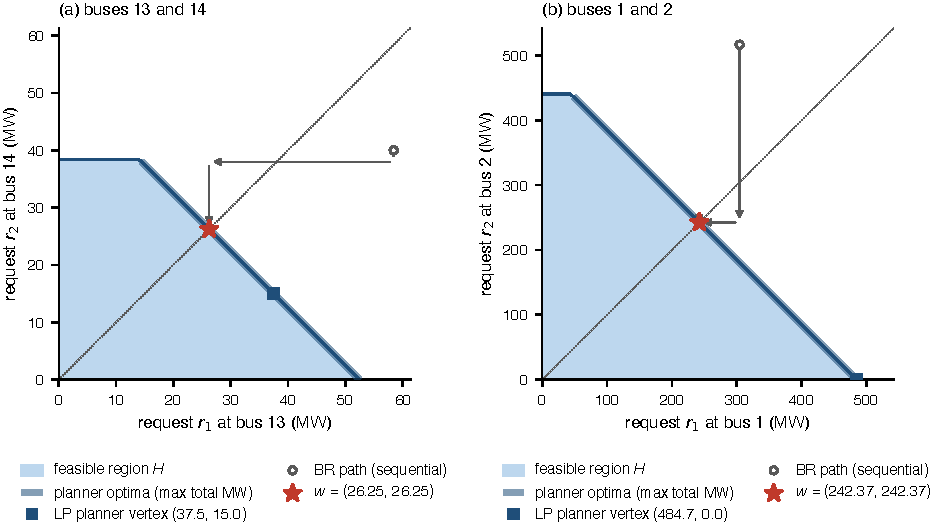
\includegraphics[width=\linewidth]{figures/ne_region_2team.pdf}
  \caption{Two teams at fixed buses. The shaded set is the team region
  $\widetilde{\mathcal H}$; the star is $w$; the thick edge is the set of
  plans with the largest total load, and the square is the planner's LP
  solution. The arrows show sequential best responses from a start outside
  the region, which reach $w$ in two moves.}
  \label{fig:ne-region}
\end{figure}

\begin{figure}[htbp]
  \centering
  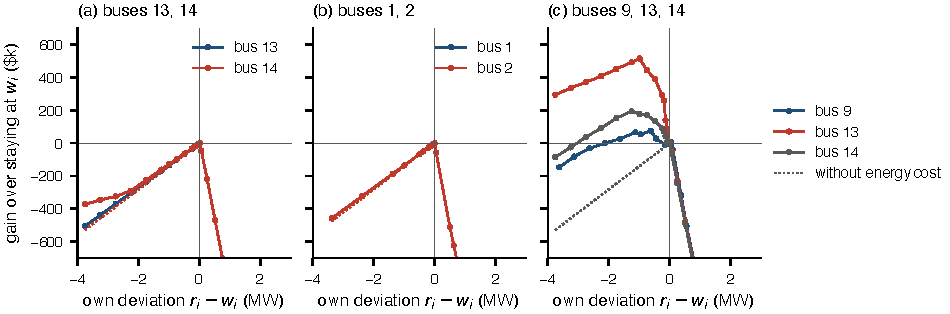
\includegraphics[width=\linewidth]{figures/ne_br_check.pdf}
  \caption{Gain from changing one team's request away from $w$, with the
  others at $w$. Solid lines charge energy at the LMP; dotted lines drop the
  energy cost, as assumption (A2) does. Every curve peaks at $w$: asking less
  loses about \$36M per MW of service, and asking more pays \$25M per MW of
  site cost for nothing. Energy cost only flattens the left side a little at
  the congested buses.}
  \label{fig:ne-br}
\end{figure}

\paragraph{Choosing the bus: two teams.} Each team chooses one of the buses
1, 2, 4, 9, 13, 14 and a request from 10\MW{} upward in steps of 10\MW{} (up to
1.3 times that bus's hosting capacity and at most 300\MW), or stays out: 114
strategies. We evaluated all 6{,}555 profiles and found every pure equilibrium
exactly (\cref{fig:ne-payoff}).
\begin{itemize}[leftmargin=*]
  \item There are three pure equilibria: both teams at bus 1 with 240\MW, or
    one team at bus 1 and the other at bus 2, each with 240\MW. Every team
    is served 235.3\MW{} (98\%) and scores \$8.04B.
  \item The equilibrium \emph{size} is unique: 240\MW{} is the grid point
    just above $w = 235.3$\MW. Asking 240 and being cut to 235.3 beats asking
    230 and being served in full, because the extra 5.3\MW{} of service is
    worth more than the extra 10\MW{} of site cost. Only the \emph{location}
    varies: on this small network the binding limit at buses 1 and 2 is the
    spare generation of the whole system, which every bus shares, and both
    buses pay the same \$30/MWh.
  \item A search for mixed equilibria (Lemke--Howson from every starting label,
    fictitious play, and replicator dynamics) found nothing new apart from a
    team mixing between bus 1 and bus 2 at 240\MW, which pays the same.
  \item The best plan on the grid for a planner, 240\MW{} at bus 1 and 230\MW{}
    at bus 4, has 1.4\% more welfare.
\end{itemize}

\begin{figure}[htbp]
  \centering
  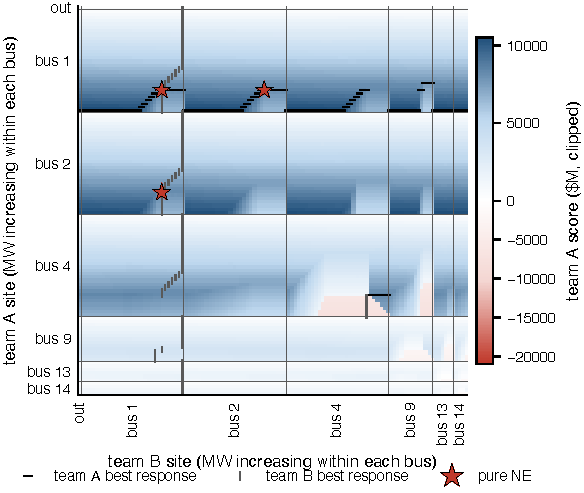
\includegraphics[width=0.75\linewidth]{figures/ne_payoff_matrix.pdf}
  \caption{Team A's score for every pair of strategies with two teams choosing
  a bus and a size. Dashes mark each team's best responses; the stars are the
  three pure equilibria, all at 240\MW{} on buses 1 and 2.}
  \label{fig:ne-payoff}
\end{figure}

\paragraph{Three and four teams.} With the same strategy grid, best-response
dynamics (each team in turn, in random order, from six random starts)
converged in three or four rounds in all twelve runs, without cycling. Every
run ended at the same exact grid equilibrium: three teams at bus 1 with
160\MW{} each, or four teams at bus 1 with 120\MW{} each. In both cases the
teams split the network's 470.7\MW{} of spare capacity equally, as
Proposition 1 predicts for one shared limit. The 50\% minimum allocation never
binds at an equilibrium; with four teams it binds briefly along several
paths, when a team overshoots and is dropped (\cref{fig:ne-dynamics}).

\paragraph{Adding a generator.} Finally we let each team add a private
generator, $G \in \{0,\ 0.25r,\ 0.5r\}$, with sizes up to 2.6 times the
bus's hosting capacity, under the game's rules: \$2.0M per MW of capital and
at most two hours of full output per day. A generator still helps, but only a
little. Against each of the three equilibria above, a team's best response is
260\MW{} with a 130\MW{} generator, which gains \$0.30B (3.8\%). From four
starts, two best-response runs converged to an exact grid equilibrium with a
small generator: both teams at bus 1 with $r = 250$\MW{} and $G = 62.5$\MW,
each served 247.7\MW. The other two kept cycling among 240\MW{} with a
60\MW{} generator, 250\MW{} without one, and 260\MW{} with 130\MW. Total
welfare rises from \$16.1B to about \$16.5B. Without the two-hour limit (and
at \$1.5M/MW) the picture was very different: both teams moved to 480\MW{}
with a 240\MW{} generator and scored \$10.9B each, because a generator that
runs every hour turns cheap fuel into \$1{,}000/MWh of served load. The
run-hour limit makes the generator what it is in practice, a device for the
few tight hours of a day.

\begin{figure}[htbp]
  \centering
  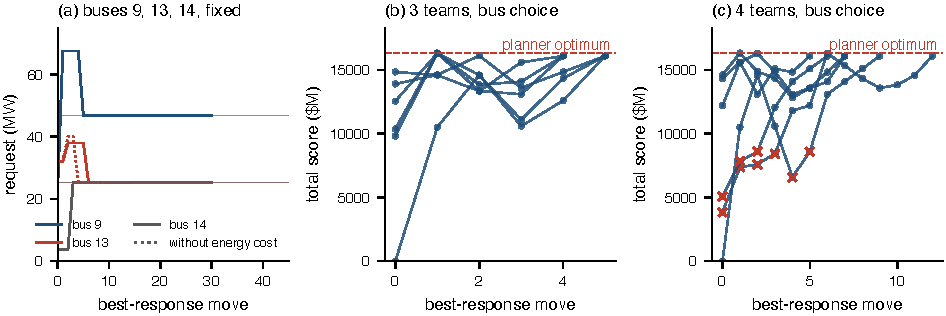
\includegraphics[width=\linewidth]{figures/ne_dynamics.pdf}
  \caption{Best-response dynamics. (a) Buses 9, 13, and 14: with and without
  energy cost, the requests settle at or right next to $w$ within a few moves.
  (b, c) Total score with three and four teams choosing buses; every run
  reaches the equilibrium on bus 1. Crosses mark profiles where a team is
  dropped by the minimum allocation.}
  \label{fig:ne-dynamics}
\end{figure}

\paragraph{What the experiments teach.}
\begin{itemize}[leftmargin=*]
  \item With the game's margin of \$36.5M per MW, the theory holds: rational
    teams ask for their equal share of the bottleneck (or the grid size just
    above it), everyone is served in full or nearly so, and the projection
    is barely used.
  \item The equal-MW equilibrium can leave capacity unused when teams sit
    behind bottlenecks of different weight (24\% in the three-team case).
  \item Energy prices at congested buses give a small incentive to ask a
    little less, but at these prices it moves requests by hundredths of a MW,
    and it matters only in Week 3.
  \item Where the binding limit is system-wide (here, generation), location
    hardly matters and teams crowd the cheapest, roomiest buses.
  \item \alert{Private generators help at the margin.} With two hours of
    output per day, a modest generator lets a team ask a little more than its
    grid share, but the best size depends on what the others do, and
    best-response dynamics may cycle. Without the run-hour limit, the largest
    generator with a request of twice the grid share would beat every other
    plan.
  \item These are results on one small network, for one submission, on finite
    grids; they illustrate the theory rather than prove it.
\end{itemize}


% ---------------------------------------------------------------------------
\section{Where the numbers come from}\label{app:numbers}

The numbers are instructional, informed by public sources and
rounded. They are not tariffs, forecasts, or ERCOT rules.

\begin{center}
\small
\renewcommand{\arraystretch}{1.15}
\begin{tabularx}{\linewidth}{@{}>{\raggedright\arraybackslash}p{0.2\linewidth} >{\raggedright\arraybackslash}p{0.2\linewidth} X@{}}
\toprule
Quantity & Value & Basis\\
\midrule
IT value & \$1,000/MWh & An instructor-chosen net margin per MWh for an AI data center, between colocation rent (about \$2.4M per MW per year, or \$270/MWh~\cite{bitdeer2026lease}) and projected GPU-cloud revenue (about \$15M per MW per year, or \$1,700/MWh~\cite{digipowerx2026gpu}).\\
Planning horizon & 10 years at 7\% & A data center runs for about ten years; per-MWh terms are discounted with the annuity factor $A = \sum_{y=1}^{10} 1.07^{-y} = 7.02$. The 7\% rate is the one OMB Circular A-4 (2003) recommended to approximate the average return on private capital~\cite{omb2003circulara4}; the 2023 revision lowered the default to 2\%~\cite{omb2023circulara4}, but private investors in data centers expect higher returns, so 7\% is a reasonable instructional choice.\\
Representative days & 5 days, 120 hours & Four medoid days from clustering the daily load profiles of one year of hourly ACTIVSg2000-based data, plus the peak-load day; weights sum to 365.\\
Site cost & \$25M/MW & Cost of building an AI data center per MW of IT load: about \$10.7M/MW for the building and up to \$25M/MW with AI fit-out~\cite{jll2026dc}, or \$21--31M/MW including servers~\cite{morganstanley2024dc}.\\
Generator capital & \$2.0M/MW & Installed cost of on-site gas engines and aeroderivative turbines for data centers, about \$1,700--2,000/kW~\cite{rabobank2026btm}; EIA reference costs are in the same range~\cite{eia2024generatorcosts}.\\
Generator cap & $G \le 0.5\,C$ & Texas SB~6 (2025) treats on-site generation that can serve at least half of a large load as backup that ERCOT may call on in emergencies~\cite{utilitydive2025sb6}.\\
Generator run hours & 2 h per day & Air permits limit on-site engines: federal rules allow 100 hours a year of maintenance and testing, of which at most 50 may be non-emergency use~\cite{ecfr6366640,sidley2025rice}, and state permits cap total operation, e.g.\ below 500 hours a year~\cite{georgia2025permit}. Two hours a day (about 730 hours a year) is a teaching choice in that range.\\
Generator operating cost & \$80/150/250 per MWh & A rising cost curve for on-site gas generation with a diesel-backup premium; the exact shape is instructional~\cite{eia2025heatrate}.\\
Storage capital & \$400k/MW + \$250k/MWh & Rounded from the 2028 moderate projection for four-hour batteries~\cite{nrel2023bess}; \$1.4M per MW of four-hour storage.\\
Grid energy price & LMP from the dispatch & The bus-level dual price of the DCOPF; about \$17--20/MWh before students add load.\\
Network & ACTIVSg2000 & Public synthetic Texas grid~\cite{activsg2000}; the load profiles are synthetic, not historical data.\\
\bottomrule
\end{tabularx}
\end{center}

% ---------------------------------------------------------------------------
\section{Working as a team}\label{app:team}

\paragraph{How to collaborate: use a private Git repository.} Commit your CSVs, scripts, and run
log so everyone works from the same files and you can always return to the
exact plan you submitted. Keep the repository private: your plan is your
competitive information.
\begin{lstlisting}[language=bash]
git init team-blue && cd team-blue
git add plans/ scripts/ runlog.csv
git commit -m "Week 2 Submission 1: plan-a, 2 sites"
git push      # to a private repository shared only with your team
\end{lstlisting}

\paragraph{Keep one candidate per folder.} The preview dispatches every CSV
in a folder together, so give each candidate its own folder:
\begin{lstlisting}
runs/
  2028-jan_jun/plan-a/plan.csv
  2028-jan_jun/plan-a.json        <- preview output
  2028-jan_jun/plan-b/plan.csv
runlog.csv
\end{lstlisting}
Large preview outputs need not be committed; the CSV and the command are enough
to recreate them.

\paragraph{Log every run.} One row per run is enough:

\begin{center}
\small
\begin{tabular}{@{}l l l l r r l@{}}
\toprule
Date & Block & Candidate & Change & Served & Score & Note\\
\midrule
10-20 & 2028 jan\_jun & plan-a & baseline & 97\% & \ldots & \\
10-20 & 2028 jan\_jun & plan-b & site 2: 40$\to$60\MW & 81\% & \ldots & below break-even\\
\bottomrule
\end{tabular}
\end{center}

\paragraph{Split the work.} For example, one person screens buses and computes
hosting capacity, one writes and checks CSVs, and one runs previews and keeps
the log. Review the final CSV together before you submit.


\addtocontents{toc}{\protect\setlength{\cftsecindent}{0em}\protect\setlength{\cftsubsecindent}{1.5em}}
\bibliographystyle{plain}
\bibliography{references}

\end{document}
